% !TEX encoding = UTF-8 Unicode
\documentclass[11pt]{article}

\usepackage[letterpaper, margin=1.5cm]{geometry}
\usepackage{graphicx}
\usepackage[english]{babel}
\usepackage[utf8x]{inputenc}
\usepackage{amsmath,amsfonts,amssymb}
\usepackage{hyperref}
\usepackage[square,numbers,sort&compress]{natbib}
\newcommand{\TODO}[1]{\begingroup\color{red}#1\endgroup}
\newcommand{\PFS}[1]{\begingroup\color{blue}#1\endgroup}
\newcommand{\CAVH}[1]{\begingroup\color{green}#1\endgroup}
\usepackage{color}
\usepackage{booktabs}
\newcommand{\tabitem}{\llap{}}
\usepackage{adjustbox}
\usepackage{longtable}
\usepackage{footnote}
\makesavenoteenv{tabular}
\makesavenoteenv{table}
\usepackage{footmisc} %reference footnotes
\usepackage{listings}
\usepackage{rotating}
%Put lines numbers in the document
\usepackage{lineno}
\linenumbers{}

\newcommand{\ADD}[1]{\begingroup\color{blue}#1\endgroup}
\begin{document}
\title{A new strategy to characterize the domain architecture structure of 
proteins of the innate inmune system in tunicate species}
% Use \titlerunning{Short Title} for an abbreviated version of
% your contribution title if the original one is too long
\author{Cristian A. Velandia-Huerto*, Ernesto Parra, Federico D. 
Brown, Adriaan Gittenberger, \\ Peter F. Stadler and Clara I. 
Berm\'{u}dez-Santana}


\maketitle

\begin{itemize}
\item \TODO{Include information about D.vexillum sequencing and assembly 
process: Clara and Ernesto.}
\item \TODO{Change everything related with another databases different to Pfam}. 
\item \TODO{Discuss about the biological meaning of the different architecture 
strategies}
\item \TODO{If yes, what is the best option to detect protein orthologs. Based 
on complete protein? or splitting  by protein domains?}
\item Adapt draft to journal template.\TODO{Which one?}. 
\end{itemize}

\section*{Introduction}

\PFS{In the last years genomes of non-model organisms have become available
  at a rapidly accelerating rate. As a consequence, their annotation and
  comparative analysis has become a task limited by time and resource
  consumption. Gene architectures serve as a convenient and relatively
  easily accessible source of information about an organism's metabolic and
  regulatory capabilities, and allow the efficient extraction of candidates
  for subsequent, more detailed functional or evolutionary studies
  \cite{aken2016ensembl,birney2004overview,ashburner2000gene,tatusov2000cog,tatusova2016ncbi}.}
  
  \PFS{Conceptually, gene annotation comprises two tasks: first the
  identification of genomic subregions that code for proteins, and second
  the assignment of functionality. Often, both issues are addressed
  simultaneously, using sequence similarity to identify homologs of a query
  with known function and the same time using homology as argument to
  transfer functional annotation. The complexity of eukaryotic genes, with
  its extensive use of alternative splicing and alternative transcription
  starts, however, makes the identification of homologs, and in particular
  the distinction of orthologs and paralogs, a non-trivial, and often
  surprisingly difficult task \cite{yandell2012}. In addition,
  homology-based annotation is by definition limited to know query sets of
  sufficiently well-characterized genes, typically from model organisms.}

  \PFS{Modern gene annotation pipelines therefore are built around
  probabilistic models that are trained on known gene structures. The first
  generation of such tools, such as \texttt{GENSCAN} \cite{genescan}
  primarily focused on promoter signals, intron/exon boundaries, and
  polyadenylation signals \cite{claverie}. State-of-the-art tools, such as
  \texttt{AUGUSTUS} \cite{augustus} or \texttt{GeneID} \cite{Blanco:2007}
  accept diverse types of training data, in particular RNA-seq based
  transcript information. The underlying model can be implemented in very
  different ways: while \texttt{AUGUSTUS} is a generalized Generalized
  Hidden Markov, a rules-based heuristic is used in \texttt{GeneID}. In the
  case of a select few model organisms, gene annotation has evolved into
  major, long-term data curation projects such as VEGA-HAVANA and GENCODE
  for the human genome. \TODO{*** Include a couple of more sentences and a
  more inclusive list of the major curation projects ***} Well curated
  gene models are in important resource also for training gene models for
  application to related species.}
  
  \PFS{The annotation of genes and open reading frames is complemented by
  systematic efforts to establish homology \-\- and in particular orthology
  \-\- information \TODO{ref}. This in turn is forms the basis for defining a
  function-based gene nomenclatures \TODO{cite HGNC}, and efforts to
  achieve a systematic, orthogy-aware nomenclature at least across some
  important clades \TODO{** mention VGNC for vertebrated **}
  \cite{aken2016ensembl, birney2004overview}. As a group, vertebrate
  genomes certainly feature the most thoroughly curated and and most
  complete functional annotation.}

In this work we focus on the sub-phylum Tunicata. As sister group of the
vertebrates they occupy a key position in the Tree of Life to understand
the prerequisites for key innovations in the vertebrate lineage. Here, we
are in particular concerned with the evolution of the immune system just
before the ``immunology big-bang'' \cite{bernstein1996} that gave rise to
the origin of the Adaptive Immune System. Like other invertebrates,
Tunicata rely on innate immunity only \cite{franchi2017}. However, they
feature a great diversity of life-styles and the world widely distribution
in ecological niches that may have forced them to evolve different immune
responses to ensure survival in their respective habitats. Since tunicates
can live as solitary sessile or pelagic or to live in colonies they have
complex relationships between the environment, so diversity in the
composition of gene of the immune system is expected
\cite{carroll2008evo,berna2014evolutionary}.

Despite the global importance of this group, genomic studies and
comparative analyses have remained scarce so far. So far only the genomes
of three solitary ascidians have been annotated in substantial depth so
far: the sessiles \textit{Ciona savignyi} and \textit{Ciona intestinalis}
mapped on its $14$ chromosomes \cite{dehal2002draft, small2007haplome} and
the pelagic \textit{Oikopleura dioica}
\cite{denoeud2010plasticity,seo2001miniature}. More recently, the genome of
a single colonial ascidians, \textit{Botrillus schlosseri} (assembled to
$13$ chromosomes) \cite{voskoboynik2013genome} has become available.
The carpet sea squirt \textit{Didemnum vexillum} has been sequenced and
analyzed for its ncRNAs \cite{velandia2016a}. To-date only a very
fragmented draft assembly is available, however.

Comparisons between tunicate and other chordate genomes have identified
both expansions of gene families but also substantial losses
\TODO{References needed}. The genomic organization of tunicates, as
exemplified by \textit{Ciona} and \textit{Oikopleura} shows substantial
differences compared to both vertebrates and amphioxus, the common outgroup
to the Olfactores \cite{delsuc2006}, and has led different authors to
formulate the idea of the existence in their evolution of processes of
genomic re-structuring in all or some tunicates genomes
\cite{putnam2008amphioxus}.  \TODO{since you say ``different authors'', we
  need several reference here!}  While the other chm.31051ordate lineages have
maintained a fairly constant rate of evolution, tunicates feature a
systematically accelerated rate of evolution which likely is linked to
specific patterns of organization of their entire gene complement
\cite{putnam2008amphioxus, berna2014evolutionary}.

We suspect, therefore, that the chordate immune system also has undergone
substantial changes, restructuring, and diversification. As a first step
towards understanding the evolution of the chordate immune system we
generate her a global overview based on the hypothesis of Paalsson \emph{et
  al.} \cite{paalsson2007building} that the immune system derives from a
small number of ancestral proteins comprising nine ancestral domains.  We
therefore focus in this survey on protein domains as the most elementary
evolutionary building blocks of the immune system and investigate the
turnover of domain architectures as a means to capture at a global level
the evolutionary driving force that led to the complexity of the immune
system in tunicates. In particular, we are interested in the emergence of
novel protein architectures throughout the Tunicata. In order to focus on
gene families that are likely associated with immune system functions, we
consider genes constructed from domains of receptors that are known to be
associated with the innate immune system. It is not uncommon in inmune
system is not rare to find copies and reshuffling of domains
\cite{Forslund2012} \TODO{more references}. We therefore employ here a
domain-based approach to homology search to overcome the limitations of
classical homology search schemes in the face of domain-level changes.

\section*{Theory}

We represent each protein $a$ as an ordered sequence $P(a)$ of domains. In
practice the domains depend on one of several annotation systems, 
\CAVH{but in this study only annotations from \texttt{Pfam} were considered}. Two 
proteins can then be compared a different levels of stringency (\CAVH{after the 
application of the domain reduction, explained in section \textit{Reduction 
System}}):
\begin{itemize}
\item[\textbf{O}rder] \TODO{What exactly is the match criterion?: Do you need
    that every domain of the query
    $Q=(Q_1,Q_2,\dots,Q_n)\in \boldsymbol{\mathfrak{G}}$ matches the
    domain list $ (P_1(a),P_2(a),\dots,P_m(a))$ of a target protein AND that
    the order is preserved? }
    \CAVH{Refers to the comparison of the $Q$ and $P(a)$ domains. It is 
required that order and the domain lists are preserved, too. Repetitions from 
query and subject are represented by one domain.}
\item[\textbf{Disorder}] \TODO{For the writing below you require that the target
    shares two distinct domains with the query list $Q$? Is this correct?
    Or do you mean that you need at least one match for all distinct
    domains and consider only hits with at least two distinct
    domains. Again I could not parse your writing below.} By construction
  every match w.r.t.\ \textbf{O} is also a match w.r.t\ \textbf{D}.
  \CAVH{The Disorder case refers to set comparisons between $Q$ and $P(a)$. 
The number of common elements ($Q \cap P(a)$) must be the same number of 
elements in $Q$ and in $P(a)$. In this case, the order does not be 
preserved.} 
\item[\textbf{Blast}] The domain-based comparisons are complemented by a simple
  \texttt{blast}-based sequence comparison between the query protein
  sequences used to construct $Q$ and the target protein
  sequence. Parameter settings are described in Materials \& Methods.
\item[\textbf{Architecture}] \TODO{I cannot understand how this is different 
from \textbf{O}.} \CAVH{Because Order and Disorder strategies works with 
proteins with $> 2$ domain types (heterodomain proteins), it is required to 
detect those candidates with only one domain family (homodomain proteins). 
Here, was used the implementation by the \texttt{RADS} program  
\cite{Terrapon:2014}. The string of domains comparisons are based on 
an identity matrix score build from Pfam v.30. It is useful to detect not only 
homodomain proteins, but also homology relations between domains with different 
accession numbers.}  
\end{itemize}

The different annotation systems and comparison methods have been integrated 
into a single workflow summarized in Figure~\ref{fig:workflow_golden}.

\begin{figure}[htb]
\begin{center}
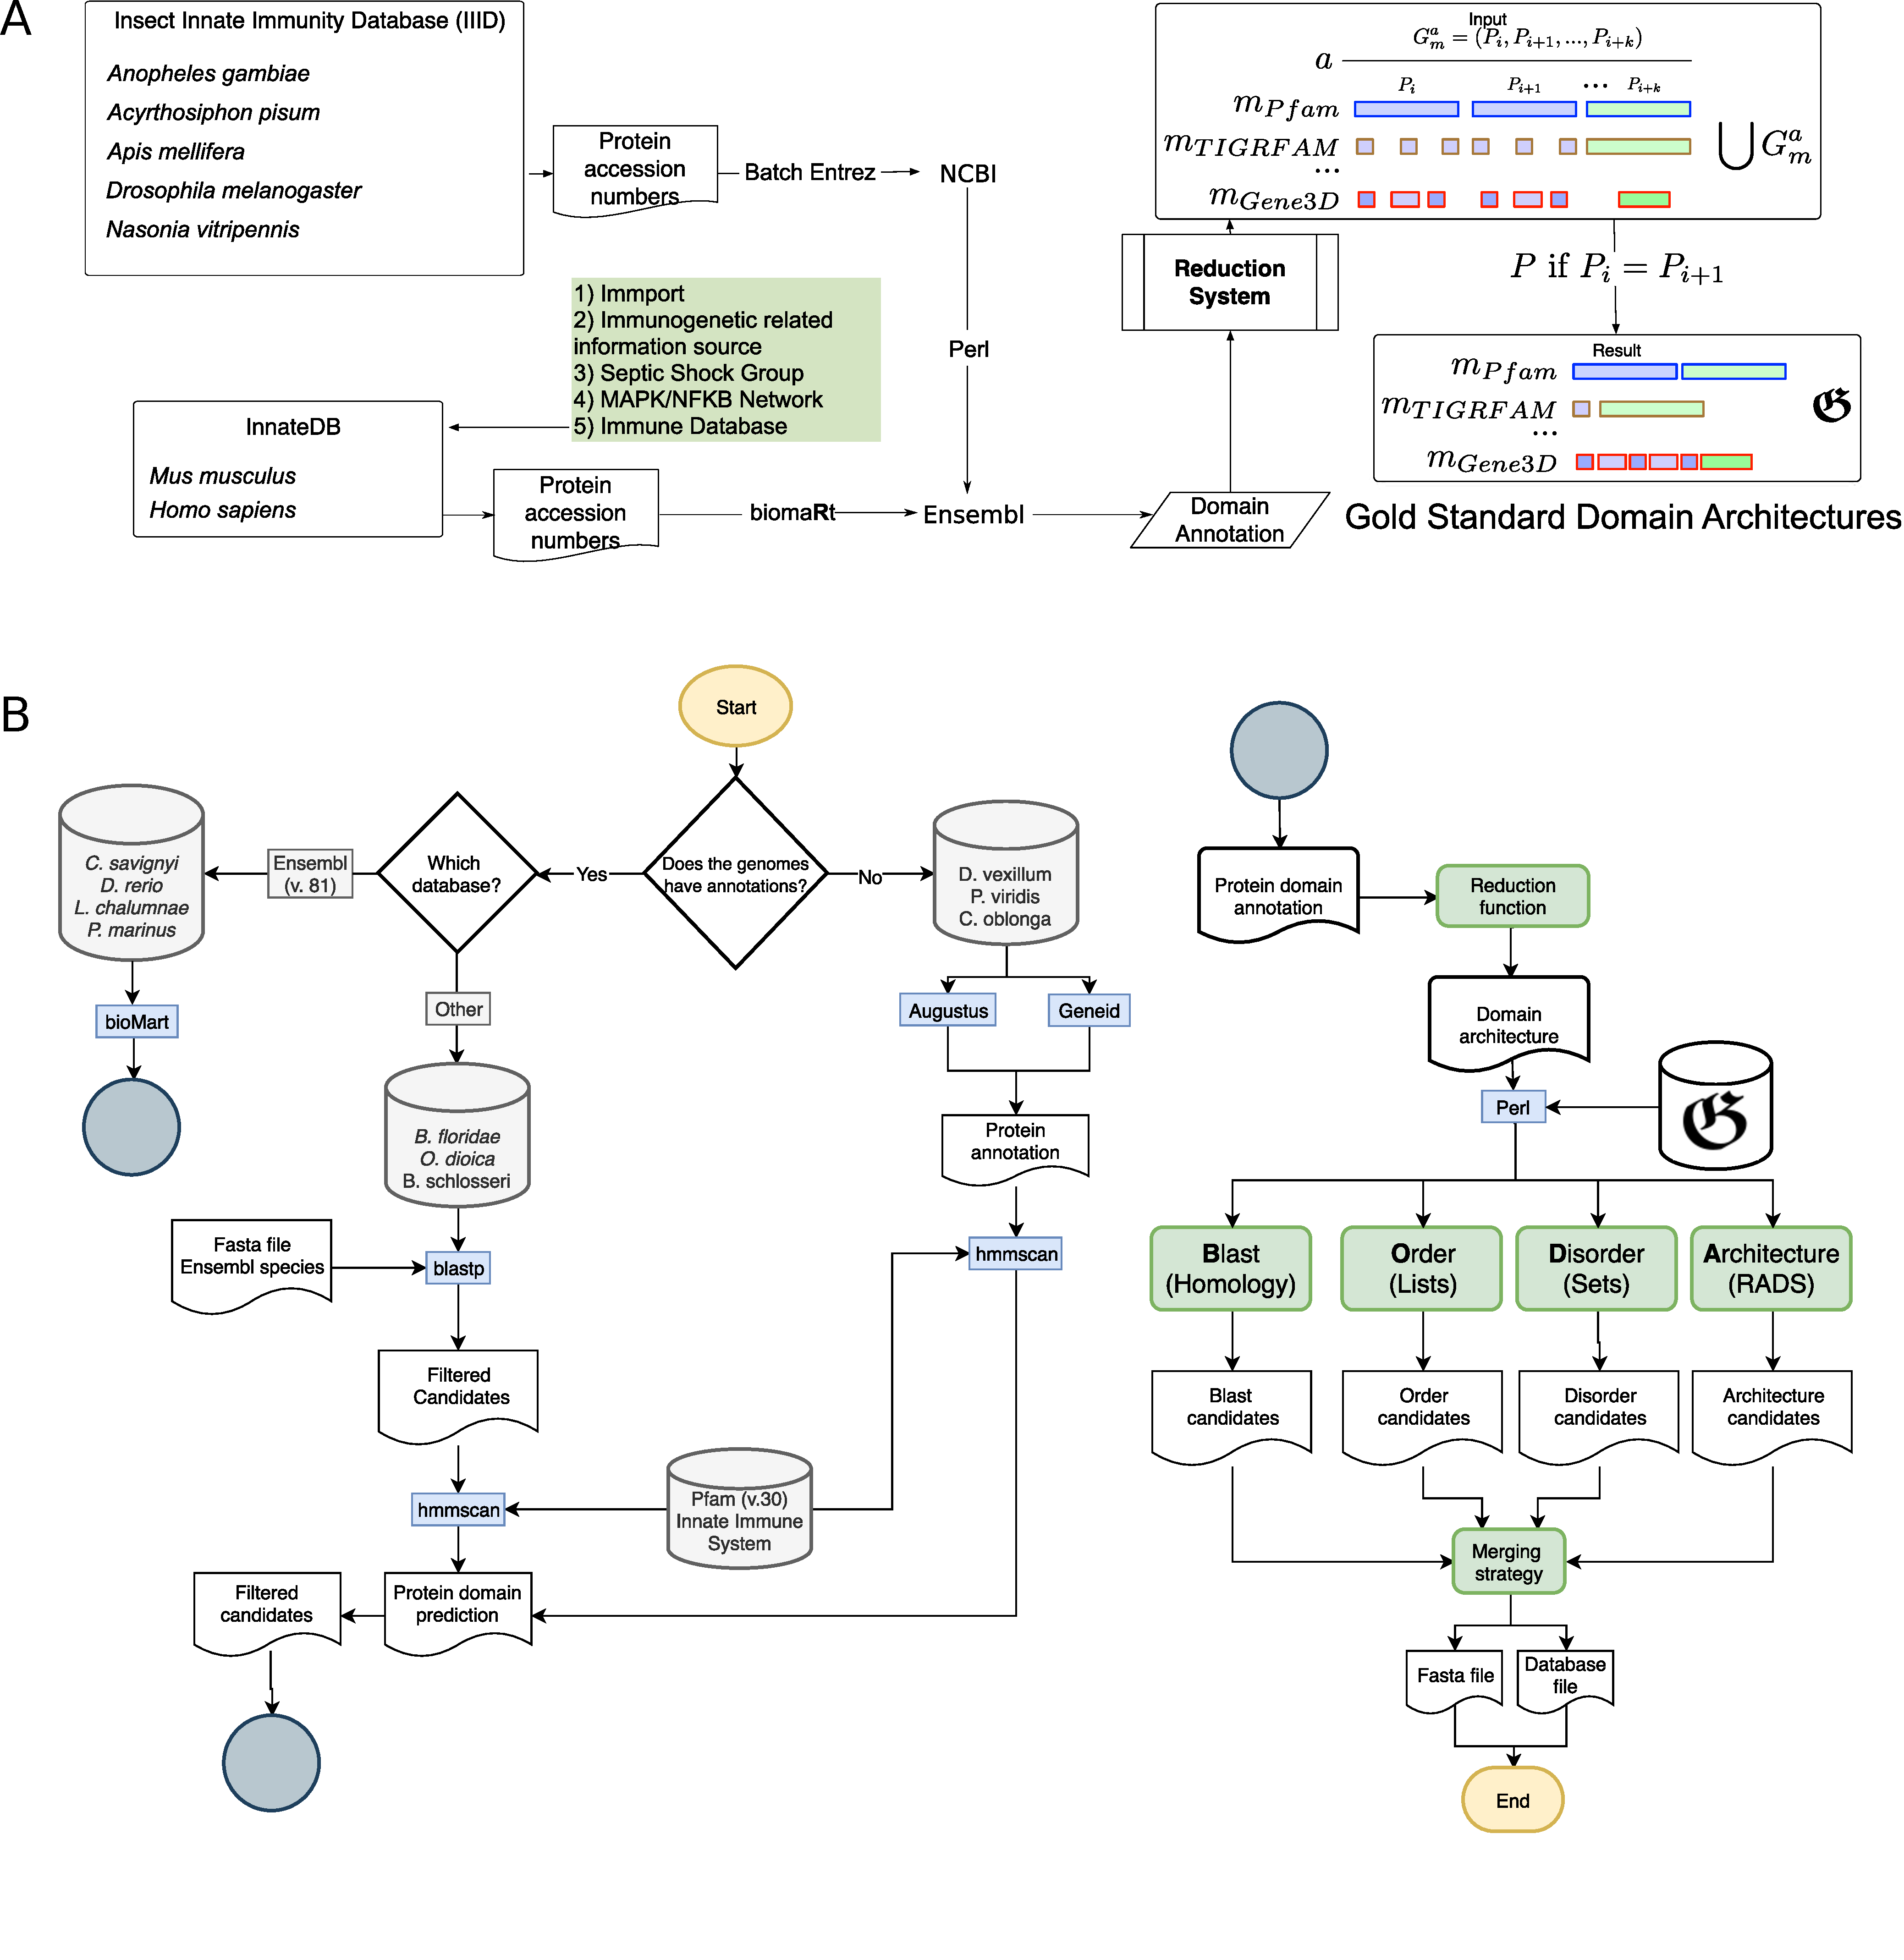
\includegraphics[scale=0.17]{figures/completeALLWorkflow3}
\caption{\textbf{A.} Workflow to generate $\boldsymbol{\mathfrak{G}}$. Innate 
immune system databases were used to obtain the accession numbers of the 
related proteins. Next, domain annotation was accesed throught \texttt{biomaRt} 
from \texttt{Ensembl} (v.81). Post processing include reduction of the 
consecutive repetitions of protein domains and finally, the definition of 
$\boldsymbol{\mathfrak{G}}$. \textbf{B.} Methodological steps to obtain innate 
immune system candidates based on $\boldsymbol{\mathfrak{G}}$ definition. 
Used programs from software packages (HHMer and blast) and in-house 
\texttt{Perl} scripts have been highlighted in blue. In green are indicated the 
\texttt{Perl} scripts that perform the reduction function and each step of 
comparison of architectures (A, B, D, O). \TODO{Clean with new and correct 
definitions.}}  
\label{fig:workflow_golden}
\end{center}
\end{figure}

\section*{Methods and Materials}

\subsection*{Comparison Strategies}\label{comparison}

List of gene architecture from tunicates and the other chordates were
greedily \TODO{what does greedily mean here?} compared with elements from
$\boldsymbol{\mathfrak{G}}$ by each $m$ using the followed strategies
\textbf{O}rder, \textbf{D}isorder, \textbf{B}last homology and
\textbf{A}rquitecture or (\textbf{O, D, B, A}) respectively.

\subsection*{Reduction system}\label{reduction}

\TODO{This subsection need complete rewriting. First the Theory section
  needs to be cleaned up.} 

To set out our work, we have defined a reference \textsl{gold standard set}. 
Our survey started building a raw set of domains as follow: let be $G^{a} = 
(P_i,P_{i+1},\ldots,P_{i+k})$ a sub-sequence of ordered domains $P$ in each 
protein $a$ of the innate immune system of organisms taking from 
\texttt{InnateDB} and \texttt{Insect Innate Immunity Database} (IIID) which have 
been annotated by \textit{Pfam} database. Since each domain $P$ has a starting 
$s_k$ and ending $e_k$ point in $a$, we defined an order $P_i \prec P_j$ if and 
only if $s_i \le s_j$. Next, we join all the domains in each protein $a$ as 
\[\bigcup G^{a}\]

Since is very commonly found copies of domains in proteins of the immune 
system, consecutive domains in $G^{a}$ were reduced to a list of unique 
representative domains $P$ if $P_i = P_{i+1}$. From now on we will refer to this 
new set as \textsl{gold standard set} $\boldsymbol{\mathfrak{G}}$ 
(Figure~\ref{fig:workflow_golden}A).
  
\subsection*{Protein domain architectures of reference}
We started with annotated and curated genes from \texttt{InnateDB} 
\cite{Breuer01012013} and \texttt{Insect Innate Immunity Database} (IIID) 
\cite{Brucker2012} in order to define a \textsl{gold standard} set of domain 
architectures of proteins of the innate immune system. At \texttt{InnateDB} many 
other immune-specific databases are linked as \texttt{Immport}, 
\texttt{Immunogenetic related information source (IRIS)}, \texttt{Septic Shock 
Group}, \texttt{MAPK/NFKB Network}, and \texttt{Immunome Database}. Our starting 
point interfaces records from \texttt{InnateDB} to \texttt{Ensembl} (v.86) 
by using \texttt{Perl} scripts and \texttt{biomaRt} R library 
\cite{Durinck:2009aa}. In this step, were mostly retrieved accession numbers 
and sequences belonging to human (GRCh38) and mouse (GRCm38) genomes. Then, to 
increase the set of gene associated with the innate immune system, the 
information from the \texttt{IIID} was used to obtain data of insects like 
\textsl{Nasonia vitripennis}, \textsl{Apis mellifera}, \textsl{Drosophila 
melanogaster}, \textsl{Anopheles gambiae} and \textsl{Acyrthosiphon pisum}. The 
latter genomes were chosen because both have annotations on \textsl{NCBI} and 
\textsl{Ensembl}. For those cases, genes annotated on \texttt{IIID} were 
retrieved using \texttt{Batch Entrez}\footnote{\url{
https://www.ncbi.nlm.nih.gov/sites/batchentrez}}. 
Accession numbers from \texttt{NCBI} were translated into the accession number 
of \texttt{Ensembl}. Then, we proceed to retrieve the data of insects in a 
similar way like in human and mouse. A reference set of domains was obtained 
independently by each domain annotation database after using a \textsl{reduction 
system} described in \textsl{Reduction function subsection}~\ref{reduction}. We 
used the \textsl{gold standard} set for further comparisons of domain 
architectures of $17$ studied species described on Additional File 1.

\subsection*{Re-assembly of \textit{D. vexillum} genome}
\TODO{Include information about re-assembly strategy from D. vexillum, 
methodological steps.}

\subsection*{Genomic data sources}

Genomic information source comes from $3$ Vertebrata species:
\textit{Petromizon marinus}, \textit{Danio rerio} and 
\textit{Latimeria chalumnae}, $10$ species of Tunicata: \textit{Oikopleura 
dioica}, \textit{Botryllus schlosseri}, \textit{Botrylloides 
leachii}, \textit{Ciona robusta}, \textit{Ciona savignyi}, \textit{Didemnum 
vexillum}, \textit{Perohora viridis}, \textit{Clavelina oblonga}, 
\textit{Molgula occidentalis} and \textit{Molgula oculata}, $1$ specie 
from Cephalochordata: \textit{Branchiostoma floridae}, represents the final set 
of chosen Chordates. As an outgroup, a set of $2$ species from Echinorderms: 
\textit{Strongylocentrotus purpuratus} and \textit{Patiria miniata} and 
additionally $1$ Hemichordate specie: \textit{Saccoglossus kowalevskii} were 
studied. The protein database sources are described in Additional File 1. 

\TODO{the following is rather incomprehensible. The concepts need to be described in the Theory sect 
see there.} 

\subsubsection*{Architecture Comparison Strategies}
\subsubsection*{\textit{\textbf{O}rder comparison}}

To trace back similar architecture organizations between annotated genes in 
tunicates with the architectures in the \textsl{gold standard set}, tunicate 
domain architectures were represented as query sets  $Q(a) = 
(\mathcal{P}_k,\mathcal{P}_{k+1},\ldots,\mathcal{P}_n)$ and are defined as a 
sub-sequence of ordered domains $\mathcal{P}$ in each protein $a$. Comparing 
the order between $P_i$s and $\mathcal{P}_i$s we defined the number 
$Q(a){success}(o)$

\begin{equation}
  Q(a){success(o)}=\left\{
  \begin{array}{@{}ll@{}}
    1, & \textsl{if}\ P_{i} = \mathcal{P}_{k} \\
    0, & \textsl{otherwise}
  \end{array}\right.
\end{equation} 

If $Q(a){success(o)} = 1$ we say that exist in $\boldsymbol{\mathfrak{G}}$ 
an architecture organization preserving order equal to an architecture 
organization $Q(a)$. If $Q(a){success(o)} = 0$ then we say those 
architectures are not related.

\subsubsection*{\textit{\textbf{D}isorder comparison}}
Since rearrangements of domains are also expected we used a second more 
flexible comparison between elements of $Q(a)$ and 
$\boldsymbol{\mathfrak{G}}$ without considering order in $\mathcal{P}$ domains. 
Now the rules are defined as follows:

\begin{equation}
  Q(a){success(d)}=\left\{
  \begin{array}{@{}ll@{}}
    %1, & Q^a_{m} \subseteq  \boldsymbol{\mathfrak{G}} \quad and \quad 
%\left|Q^a_{m}\right| \geq 2 \\ Re-defined it was wrong written.
    1, & \left|Q^a \cap \boldsymbol{\mathfrak{G}}\right| = 
\left|Q^a\right| = \left|\boldsymbol{\mathfrak{G}}\right| \quad and \quad 
\left|Q^a\right| \geq 2 \\
    0, & \textsl{otherwise}
  \end{array}\right.
\end{equation}

If $Q(a){success(d)} = 1$ we say that exist in $\boldsymbol{\mathfrak{G}}$ 
an architecture composition similar to an architecture organization $Q(a)$. 
If $Q(a){success(d)} = 0$ then we say those architectures are not related. 
Note that here the order of domains  is not a constrain to classify a query set 
$Q(a)$ as success.

\subsubsection*{\textbf{B}last homology comparison}
A classical homology strategy with \texttt{blastp} was used \cite{Korf:2003}. 
For these homology searches, pairwise comparisons were done between the 
proteins used to built both query and \textsl{gold standard} sets. After running 
BLAST following the combination of parameters: 
\begin{lstlisting}[language=bash, breaklines=true]
blastall -p blastp -d <DB> -i <QUERY> -f 9 -F `m S' -M BLOSUM45 -e 100 -b 
10000 -v 10000 -m 8
\end{lstlisting}

were filtered candidate homologous if they satisfied:
\begin{itemize}
\item E-value $\leq 0.001$.
\item Coverage to query length $\geq 60$\%.
\item Identity $\geq 30$\%.
\end{itemize}

\subsubsection*{\textbf{A}rquitecture comparison}
Before the application of reduction system, there are different 
architectures composed by only one domain that had not been taken into account 
with the O,D,B strategies. In order to complement the search strategies, a
comparison between \textsl{gold standard} architectures and query architectures 
was performed applying the methodology reported 
by \texttt{RADS}\footnote{http://domainworld.uni-muenster.de/programs/rads/}\cite{Terrapon:2014}.

First, a domain architecture database was created with the \textsl{gold standard} domains using the program:
\begin{lstlisting}[language=bash, breaklines=true]
makeRadsDB -i <DOMAIN-DISTRIBUTION1> <DOMAIN-DISTRIBUTION2> -s <Seqfasta1> <Seqfasta2> seqFile2.fa -o <OUT-DB>.
\end{lstlisting}

And the comparison was applied against all the query architectures with: 

\begin{lstlisting}[language=bash, breaklines=true]
rads -c -d <DB> -m <Matrix> -q <Input> -o <OUTFILE>
\end{lstlisting} 

Where DB corresponds to the output file from \texttt{makeRadsDB}. Matrix file 
(pfam-30.dsm) was obtained directly from \texttt{RADS} site; Input file 
correspond to the domain's distribution organised as pfam\_scan output 
file. Final candidates were retrieved if reported a similarity normalized score $\geq 0.75$.

\subsection*{Merging output of comparison strategies}
In order to identify the best candidates to be related with the immune 
system, all the previously results from Order, Disorder, Blast and Architecture 
strategies were merged and combined with a \texttt{Perl} script. Candidates 
that have been detected only by Blast (B) strategy were not taken into 
account. Considering all other possible combinations of strategies, it is 
important to note that $O \subset D$, it means that combinations as O, OB, OA, 
OBA are not possible. In this way the remaining combinations $10$ were 
considered to detect the candidates for the innate immune system.

\subsection*{Cleaning specific Hidden Markov Models (HMMs) for each 
domain}
Specific Hidden Markov Models (HMMs) for each domain on the different 
annotation sources were obtained using the program \texttt{hmmfetch} by 
screening on \texttt{Interpro} (Version 60). Then HMMs related with innate 
inmune system in $\boldsymbol{\mathfrak{G}}$ were retrieved. The final list was 
used in further steps.

\subsection*{Screening of architectures domains in Ensembl-non-annotated 
tunicate and cephalochordate species}

\subsubsection*{Ensembl-non-annotated genomes}

The protein annotation for the cephalochordate \textsl{B. floridae} and 
the tunicates \textsl{O. dioica} and \textsl{B. schlosseri} are based on the 
scheme reported at \texttt{JGI Genome Portal} 
(\url{http://genome.jgi.doe.gov/Brafl1/Brafl1.download.ftp.html}) for \textsl{B. 
floridae}, \texttt{Oikoarrays} 
(\url{http://oikoarrays.biology.uiowa.edu/Oiko/Downloads.html}) for \textsl{O. 
dioica} and \texttt{ANISEED} database 
(\url{http://www.aniseed.cnrs.fr/aniseed/download/download_data}) for \textsl{B. 
schlosseri}. In first place, candidates related to the immune system in the 
species \textit{C. robusta}, \textsl{C. savignyi}, \textsl{L. chalumnae}, 
\textsl{P. marinus} and \textit{D. rerio} were used as query sequences to 
perform pairwise homology searches with \texttt{blastp}.

\begin{lstlisting}[language=bash, breaklines=true]
blastall -p blastp -d <DB> -i <QUERY> -F `m S' -m 8 -o <OUT_FILE>
\end{lstlisting}

After filtering, hits candidates with high level of similarity were 
considered as a set of putative candidates, as described below:

\begin{itemize}
\item E-value $\leq 0.001$
\item Coverage $\geq 60$ \%
\item Identity against query $\geq 30$\%.
\end{itemize}

After that, an exhaustive search of HMM domains was conducted by the suite 
\texttt{HMMer} to detect domains using the mapped HMMs in 
$\boldsymbol{\mathfrak{G}}$. Best candidates to annotate protein domains 
derived from \texttt{PFAM} was obtained filtering all of the candidates that 
reported a bitscore $\geq$ Gathering cut-off from \texttt{Pfam} (v.30) and 
reported an internal i-E-value and c-E-value $\leq 0.01$. For the inference of 
domain architecture in these proteins, previously described approach had been 
applied, including the comparison against the \textsl{gold standard} set. The O, 
D, B and A strategies were merged generating the candidates that were 
overlapping between all the strategies, as described on Figure 
~\ref{workflow_golden}.

\subsubsection*{Draft genomes without annotation}

For the recently reported draft genomes of \textit{C.\ oblonga} and 
\textit{P.\ viridis} a \textit{de novo} gene prediction was performed 
directly on the assembled contigs using \texttt{GeneID}\cite{Blanco:2007} 
with the following parameters:

\begin{lstlisting}[language=bash, breaklines=true]
geneid -3 -P <Parameter file> <FASTA FILE> -A >> <GFF3 file>
\end{lstlisting}

Here the \textit{Parameter file} was fetched via \texttt{FTP} for the 
tunicates: \textsl{C. intestinalis}\footnote{
ftp://genome.crg.es/pub/software/geneid/cintestinalis.param\_Apr\_26\_2006} and 
\textsl{O.dioica}\footnote{
ftp://genome.crg.es/pub/software/geneid/odioica.param\_Nov\_10\_2006}. The final 
result was a \texttt{GFF3} file describing the coordinates on the candidate 
genes, and additionally the set of possible protein candidates in a 
\texttt{fasta} format. Over those candidates \texttt{HMMer} was ran to detect 
domains that intersect with the mapped HMMs in $\boldsymbol{\mathfrak{G}}$. 
Again, filters by each $m$ was used, the \textsl{Reduction 
system}~\ref{reduction} step and comparison strategies \textbf{O, D, B, A} were 
done (Figure~\ref{workflow_golden}).

For the draft genome of the carpet sea squirt \textit{D. vexillum} 
\cite{velandia2016a} a \textit{de novo} gene prediction was performed 
directly on the assembled contigs using \texttt{AUGUSTUS} \cite{augustus} 
with the following parameters:

\TODO{Put AUGUSTUS parameters}

and the complete prediction of homologous architectures was obtained applying 
the pipeline \TODO{Name of my pipeline!}.

%\subsection*{Identification of Nucleotide coordinates and CDS sequences from 
%Protein Domains}
%The nucleotide sequences and the genome coordinates were retrieved for 
%each protein domain that belongs from homologous architectures, inferred from 
%the comparison strategies against \textsl{gold standard}. As shown in Figure 
%~\ref{proteindomains2cds}, the required steps to infer this information for the 
%majority of domains, relies on CDS sequences and annotations at genome level. 
%In 
%case of \textsl{O. dioica}, \textsl{B. schlosseri} and \textsl{B. floridae}, 
%\texttt{GFF} files where downloaded from correspondent databases, including 
%their reported fasta files. In case of \textit{D. vexillum}, the CDS fasta 
%files 
%were inferred directly from the \texttt{GFF} file through a \texttt{Perl} 
%script. For species annotated on \texttt{Ensembl}, transcripts fasta files for 
%each species on their correspondent \texttt{FTP} site\footnote{As described on 
%http://jul2015.archive.ensembl.org/info/data/ftp/index.html} were obtained. 
%With 
%all fasta files from transcripts or CDS, required indexed fasta files were 
%generated with \texttt{makeblastdb}. Fasta sequences from previously 
%identified 
%domains in each candidate proteins were obtained, using \texttt{tblastn} were 
%compared in a pairwise alignment against their correspondent CDS sequences, as 
%described below:

%\begin{lstlisting}[language=bash, breaklines=true]
%tblastn -db <CDS_DB> -query <PROTEIN_DOMAINS_FASTA> -evalue 1000 -word_size 6 
%-window_size 40 -comp_based_stats 2 -gapopen 11 -gapextend 2 -matrix 
%BLOSUM62 -db_gencode 1 -seg no -threshold 21 -outfmt 6 -out <OUT_FILE>
%\end{lstlisting}

%Tabular results were filtered applying the following conditions:

%\begin{itemize}
%\item The name of the possible candidate have to be equal to the 
%previous name of the transcript which it was reported for this protein.
%\item The identity have to be equal to $100$\%. 
%\end{itemize}

%In order to identify the genomic coordinates from these identified CDS, a 
%\texttt{blastn} strategy was applied against the respective reported gene as 
%follows: 

%\begin{lstlisting}[language=bash, breaklines=true]
%blastn -db <Genes DB> <DOMAINS FASTA> -num_threads 8 -evalue 1e^20 -word_size 
%9 
%-gapopen 2 -gapextend 5 -penalty -3 -reward 1 -dust yes -outfmt 6 -out 
%<OUT_FILE>
%\end{lstlisting}

%Specific filters for this methodology were designed (as show below) and the 
%final candidates were organized in a GFF file for each protein database.

%\begin{itemize}
%\item The name of the possible gene candidate have to be equal to 
%the previous name of the gene which it was reported for this CDS or transcript.
%\item The identity have to be equal to $100$\%. 
%\end{itemize}


%\begin{figure}[htbp]
%\begin{center}
%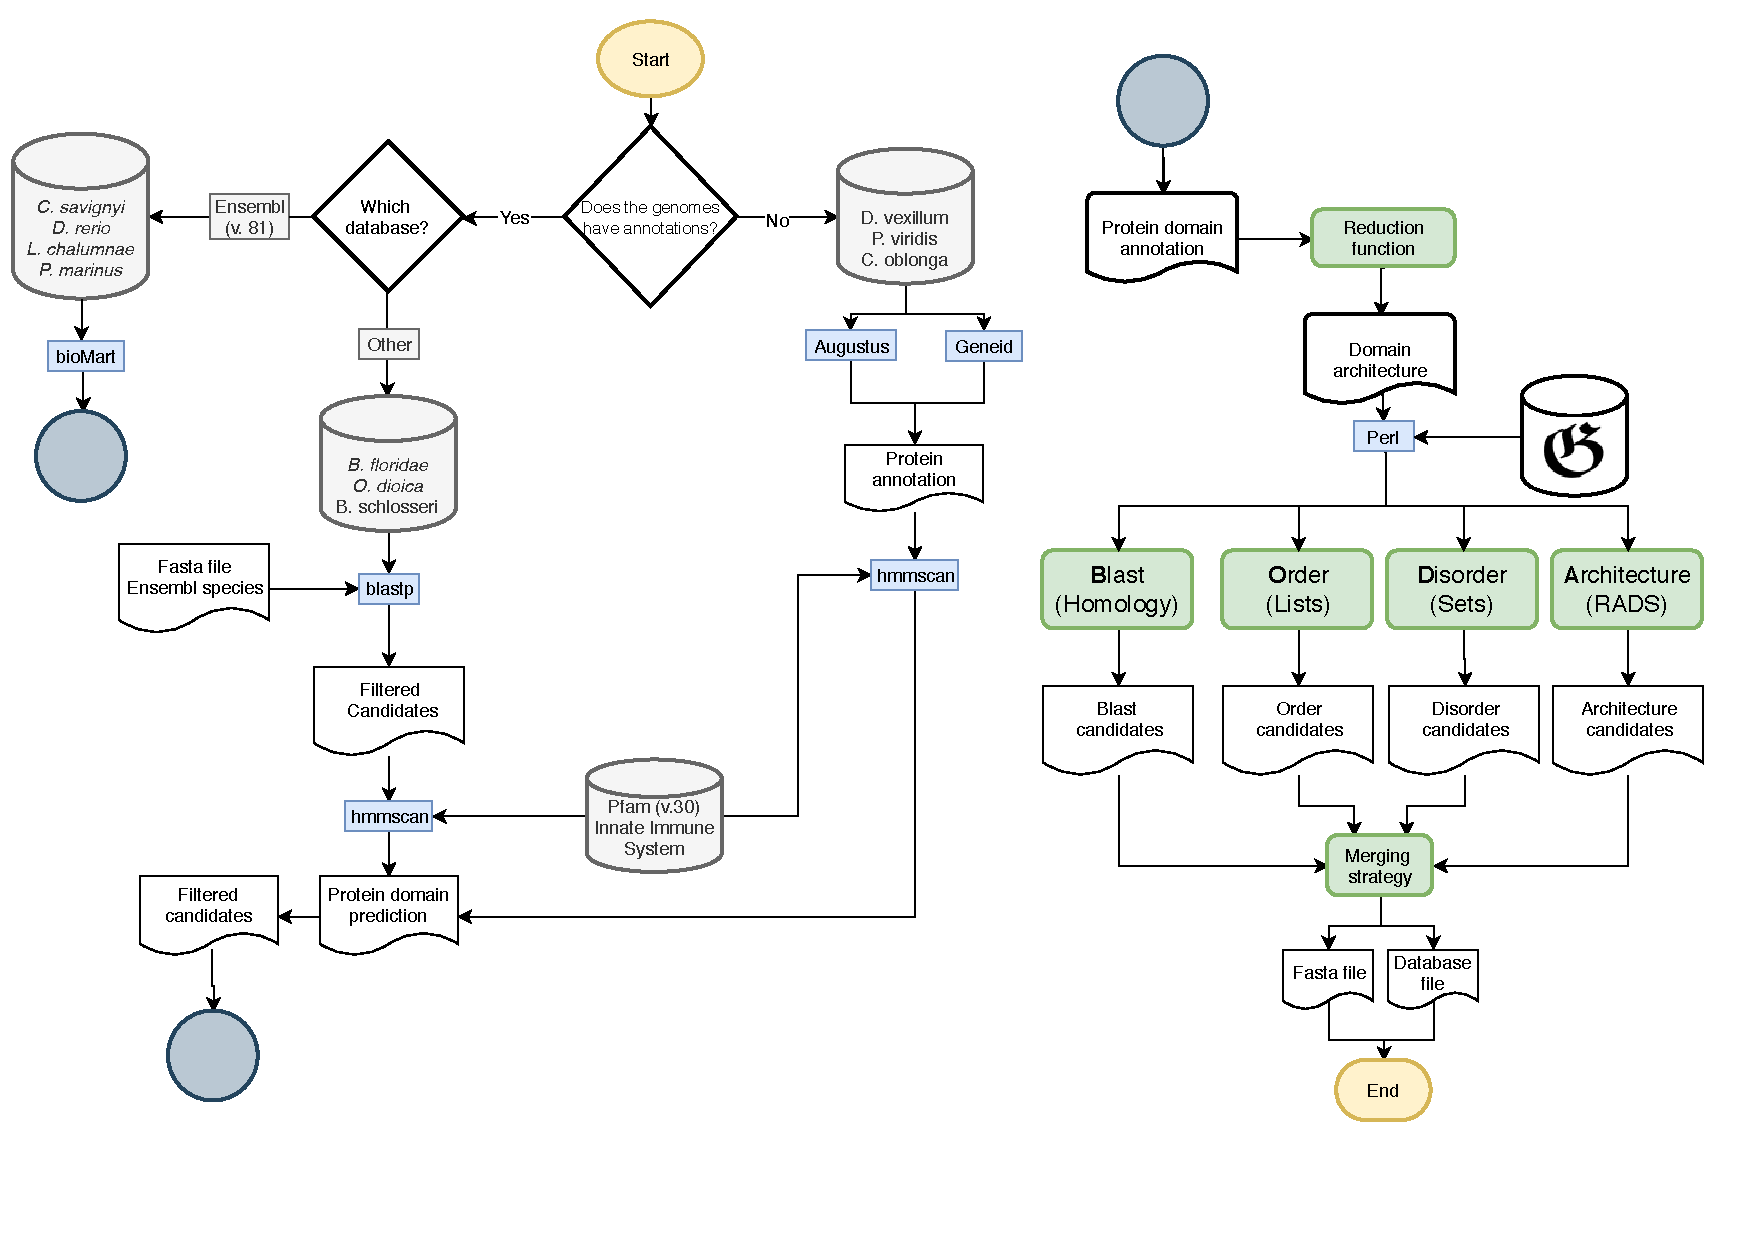
\includegraphics[scale=0.45]{figures/workflowComplete}
%\caption{Methodological steps to obtain innate immune system candidates. 
%Have been highlighted in blue the programs used in this pipeline. In green, 
%those scripts in \texttt{Perl} that performed the reduction function and each 
%of the architecture comparison considered in this study.}
%\label{workflow_domains}
%\end{center}
%\end{figure}

%\begin{figure}[htbp]
%\begin{center}
%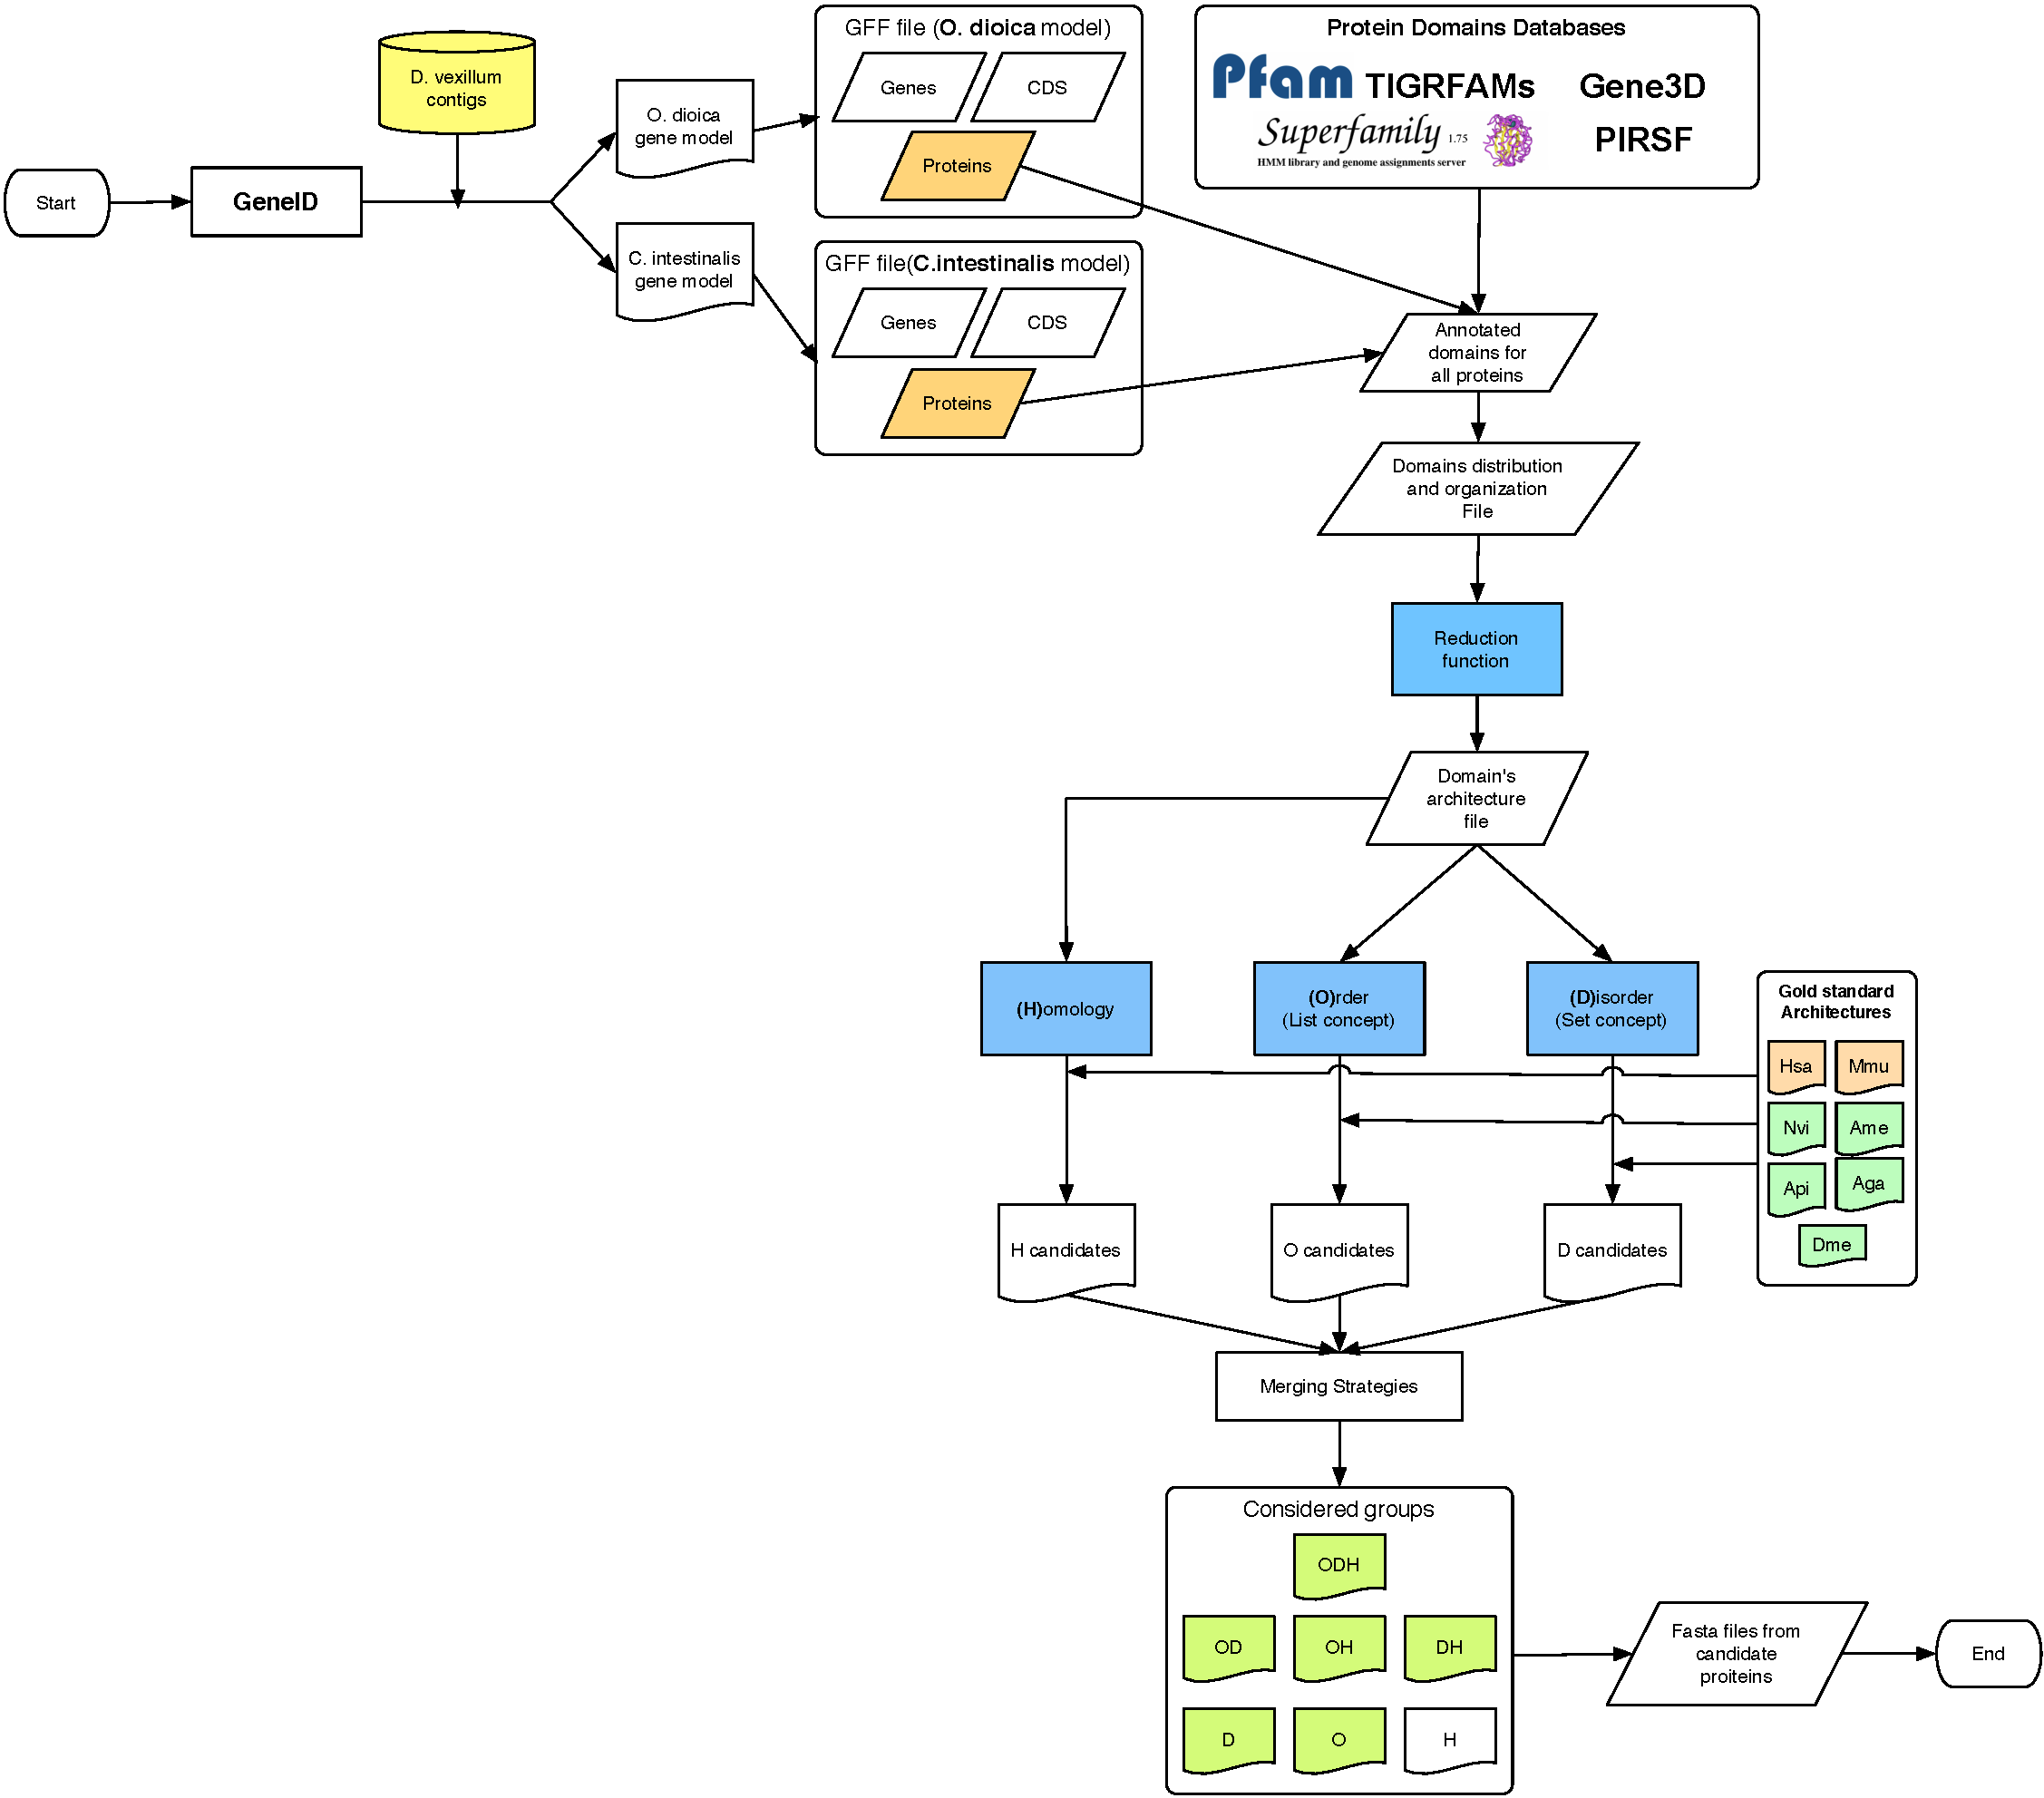
\includegraphics[scale=0.3]{figures/workflow_2_dvex}
%\caption{Designed workflow to annotate genes \textit{de novo} in \textit{D. 
%vexillum} genome, and subsequently obtain the architecture distributions 
%according to \textbf{O}rdered, \textbf{D}isorder and \textbf{B}last strategy.}
%\label{workflow_domains_dvex}
%\end{center}
%\end{figure}

%\begin{figure}[htbp]
%\begin{center}
%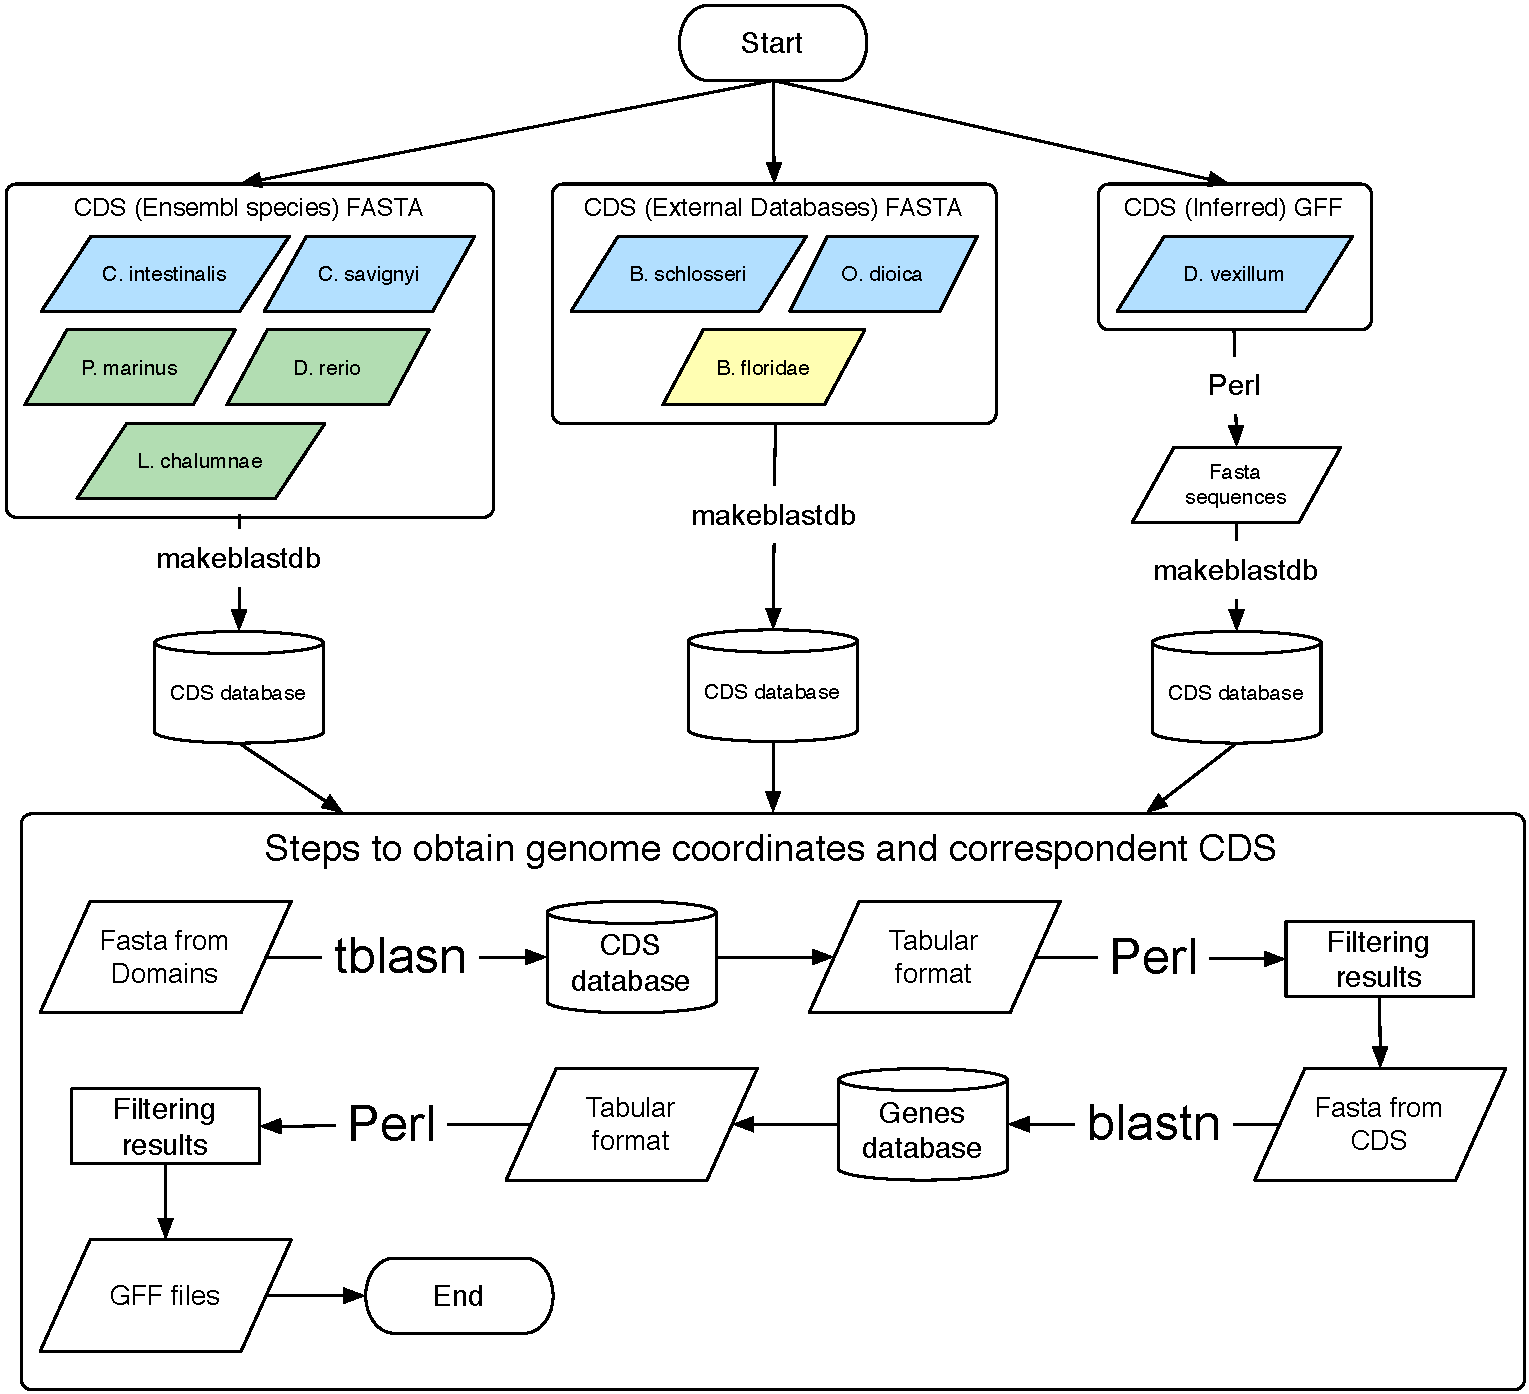
\includegraphics[scale=0.3]{figures/prot2cds}
%\caption{Designed workflow to annotate genes \textit{de novo} in \textit{D. 
%vexillum} genome, and subsequently obtain the architecture distributions 
%according to \textbf{O}rdered, \textbf{D}isorder and \textbf{B}last strategy.}
%\label{proteindomains2cds}
%\end{center}
%\end{figure}

\subsection*{Orthology detection between candidate innate immune system 
proteins}
In order to detect orthologous groups among innate immune system candidates, 
proteins that reported the same architecture relationships respect to the gold 
standard proteins, were compared using \texttt{ProteinOrtho} (v.5.16) \cite{Lechner2011}, 
as follows:

\begin{lstlisting}[language=bash, breaklines=true]
proteinortho5.pl -force -graph -clean -keep -project=<name-project> 
-step=1 <fasta files>
proteinortho5.pl -force -graph -clean -keep -step=2 
-project={name-project} <fasta files>
proteinortho5.pl -force -graph -clean -keep -step=3  
-project=<name-project> <fasta files>
\end{lstlisting}

As described earlier (Figure~\ref{fig:FrecEstrat}A), studied species could be grouped
into $5$ clades: echinorderms, hemichordates, cephalochordates (CE), tunicates (TU) and vertebrates 
(VE); which have been used as a reference to make orthology comparisons. In this case, the species that belong
from echinoderms and hemichordates have been designed as \textsl{Outgroup} (OU) and 
$\boldsymbol{\mathfrak{G}}$  species (GO) have been always considered, in order to create orthology
comparisons as follows:
\begin{itemize}
 \item TTO1: OU, CE, TU, VE, GO (All species and Golden).
 \item TTO2: CE, TU, VE, GO (Chordata and Golden).
 \item TTO3: CE, TU, GO (Cephalochordata, Tunicata and Golden).
 \item TTO4: TU, VE, GO (Vertebrata, Tunicata and Golden).
 \item TTO5: TU, GO (Tunicata and Golden).
\end{itemize}

For all of the defined treatments (TTOs), detected 1:1 and co-orthologous relationships between 
pre-defined architecture groups of orthology were obtained with a \texttt{Perl} script.

At the same time, available annotation from $\boldsymbol{\mathfrak{G}}$ were obtained from 
\texttt{Ensembl} using \texttt{biomaRt}.For protein candidates that belongs from studied 
species and shared orthologous relations with a $\boldsymbol{\mathfrak{G}}$ protein, the 
retrieved annotation from from \texttt{Ensembl} and \texttt{Interpro} accession numbers were 
associated and reported.

\subsection*{Gain and losses of domains}

Reconstruction of family history using Dollo's parsimony was achieved with \texttt{Count} \cite{csuros2010}, using the orthology results. The presence/absence matrices were obtained using
a \texttt{Perl} script and the The phylogenetic distribution of this species 
were obtained from \TODO{[71]} for tunicates, and for the other organisms from 
Ensembl compara \TODO{[72]}.

\section*{Results}

\subsection*{Global distribution of domains}

A total of $8846$ annotated genes associated with the innate immune system were retrieved 
from \texttt{InnateDB}, of which $7043$ and $1803$ belong to human and mouse 
respectively. After interfaced these records with Ensembl Genome Browser a total 
of $35136$ and $5179$ proteins were identified. Next, to integrate annotations from
the source \texttt{Insect Innate Immunity Database} (IIID) a total of $1312$ proteins were
recovered and were accessed as follows: \textsl{N. vitripennis} $393$ ($368$), 
\textsl{A. mellifera} $170$ ($106$), \textsl{D. melanogaster} $298$ ($242$), \textsl{A. gambiae}
$366$ ($333$) and \textsl{A. pisum} $85$ ($81$), the number in parenthesis corresponds to 
the \textsl{bone fide} annotation in \texttt{Ensembl}. Finally the domain structure was 
traced back with \texttt{biomaRt} in \texttt{Ensembl}. Then, as described in Additional 
File 2, \textsl{gold standard} set ($\boldsymbol{\mathfrak{G}}$) was conformed.

\subsection*{\textbf{ABDO} strategy comparisons of domains}\label{subODB}

The number of genes and proteins that have been included into $\boldsymbol{\mathfrak{G}}$ 
is described in Additional File 2: Table 1. In general, most of the current 
annotations belongs from human ($84.74$\%) and mouse ($12.51$\%) and inside the 
annotation of insects, \textit{N. vitripennis} ($33.14$\%) is the most frequent. 
Those candidates were used as query arquitectures that have been compared through previously 
described \textbf{ABDO} strategies to the subject species (Additional File 1: Table1). 
Taking advantage of the current annotation state is possible to group the query 
species as follows: 1.\ those ones that have been annotated in \texttt{Ensembl} as
\textit{C.\ robusta}, \textit{C.\ savignyi}, \textit{P.\ marinus}, \textit{D.\ 
rerio} and \textit{L.\ chalumnae}. Also, 2.\ those that have gene and protein annotations 
but, in independent databases and without the prediction of domains, like \textit{B.\ floridae}, 
\textit{B.\ schlosseri} and \textit{O.\ dioica}. The 3.\  group is composed by those 
genomes that have a \textsl{de novo} assembly, as: \textit{D.\ vexillum}, \textit{C.\ oblonga} and 
\textit{P.\ viridis}, which did not reported predictions of genes or proteins, then this 
prediction were performed as described in \textsl{Methods and Materials} with the 
\texttt{GeneID} program using the previously constructed gene models from 
\textit{C.\ robusta} and \textit{O.\ dioica}\footnote{For those genomes, in Table 
~\ref{table:distribution_prot} are referenced as \textsl{Ciro} and \textsl{Oidi} in parenthesis,
respectively} and with \texttt{AUGUSTUS} for \textit{D. vexillum}. Finally, the last group 4.\ 
is composed by the outgroup species from hemichordates: \textit{S.\ kowalevskii} and from 
echinoderms: \textit{P.\ miniata} and \textit{S.\ purpuratus} and the species from 
tunicates that have available annotations from protein sequences (\textit{M.\ occidentalis}, 
\textit{M.\ oculata} and \textit{B.\ leachii}) where the \textbf{ABDO} predictions have 
been calculated applying the automated pipeline \TODO{NAME\_PIPELINE} generated in this study.

Current annotation of genes and proteins could reflect the state of assembly
or annotation efforts on subject species. As pointed out in Table~\ref{table:distribution_prot}
is possible to calculate a relationship between the distribution of annotated genes ($g$) and 
their protein-coding products ($p$), as:
$p/g$. 

For \textit{P.\ miniata}, \textit{B.\ floridae}, \textit{O. dioica}, 
\textit{B.\ schlosseri} and \textit{B.\ leachii}, this number reflect an 1:1 relation, indicating
that the annotation for genes are strictly limited for protein-coding. Larger numbers of 
proteins have been detected on \textit{de novo} predictions of genes strategy, where the genomes 
from \textit{C.\ oblonga} and \textit{P.\ viridis} reported higher number of possible protein
products. After retrieving or predicting the protein domain annotation, a reduced number of 
proteins with domains could be identified, specifically for aforementioned genomes, less than
$1\%$ of those results had a succesfull domain annotation. Next with these subset of proteins,
domain architectures could be identified, appliying the \textsl{Reduction function} described 
earlier. After independent methods of comparison againgst $\boldsymbol{\mathfrak{G}}$, the 
number of candidates are described for each homology architecture strategy (\textbf{ABDO}).
The final number of innate immune system proteins set is described on column \textbf{Total Prot. 
ISS}, which was obtained after merging steps on the ABDO results. 
%Following values based on the calculated numbers from: supportFileProteins.xlsx
When all the strategies were applied, always the B strategy reported higher 
frequencies of protein candidates in comparison to the O or D. Those 
results are more similar to the A strategy, which does not have a previous 
reduction step. In overall, those results show a highest distribution from 
annotated immune system proteins in vertebrates (median = $53.06$\% $\pm 
2.91$, n=3), in comparison to tunicates (median = $27.15$\% $\pm 20.97$, n=12), 
cephalochordates ($16.69$\%, n=1), and the outgroup composed by hemichordates 
($41.32$\%, n=1) and echinoderms (median = $43.85$\% $\pm 12.08$, n=2). High 
standard deviation in tunicates are a consequence of the inclusion of the new 
draft genomes (from \textit{C.\ oblonga} and \textit{P.\ viridis}), where the 
prediction of genes was \textsl{de novo} by \texttt{GeneID}. In this context, 
only considering the tunicates genomes that had a previous annotation, the 
estimated values changed: (median =$36.65$\% $\pm 13.55$, n=8). Specifically,
\CAVH{inside this clade, through colonial (median=$37.28$\% $\pm 18.57$) and solitary 
($37.92$\% $\pm 11.98$) tunicates there is not significant differences on the 
medians (Kruskal-Wallis rank sum test, $p=0.8815, \alpha=0.05$).}

\TODO{Please correct the table and improve the discussion} 

\begin{sidewaystable}
\small
\centering
\begin{tabular}{p{3.2cm}p{2cm}p{2cm}p{2cm}p{2cm}p{2cm}p{2.1cm}p{2.7cm}p{2.6cm}}
\toprule
\textbf{Specie}&\textbf{Annotated Genes}&\textbf{Annotated Proteins}&\textbf{Annotated Prot with domains}&\textbf{Orderded Prot}&\textbf{Disorder Prot}&\textbf{Blast Prot}&\textbf{Architecture}&\textbf{Total Prot IS} \\ 
\midrule
\textsl{P. miniata}&    $30399$&$30399$&$20192$ ($66.42$)&$1936$ ($6.37$)&$2161$ ($7.11$)&$11577$ ($38.08$)&$17006$ ($55.94$)&$17151$ ($56.42$)\\
\textsl{S. purpuratus}& $33663$&$35786$&$23640$ ($66.06$)&$3248$ ($9.08$)&$3542$ ($9.90$)&$15420$ ($43.09$)&$19811$ ($55.36$)&$19964$ ($55.79$)\\
\textsl{S. kowalevskii}&        $32367$&$22111$&$14888$ ($67.33$)&$1973$ ($8.92$)&$2152$ ($9.73$)&$9737$ ($44.04$)&$12398$ ($56.07$)&$12505$ ($56.56$)\\
\midrule
\textsl{B. floridae}&   $50817$&$50817$&$25430$ ($50.04$)&$5499$ ($10.82$)&$4183$ ($8.23$)&$21767$ ($42.83$)&$21000$ ($41.32$)&$8480$ ($16.69$)\\
\midrule
\textsl{O. dioica}&     $17212$&$17212$&$5709$ ($33.17$)&$1342$ ($7.80$)&$955$ ($5.55$)&$4577$ ($26.59$)&$4797$ ($27.87$)&$4808$ ($27.93$)\\
\textsl{M. occidentalis}&       $30639$&$33023$&$13050$ ($39.52$)&$1195$ ($3.62$)&$1281$ ($3.88$)&$7170$ ($21.71$)&$11192$ ($33.89$)&$11243$ ($34.05$)\\
\textsl{M. oculata}&    $15313$&$16616$&$9985$ ($60.09$)&$1336$ ($8.04$)&$1419$ ($8.54$)&$6615$ ($39.81$)&$8472$ ($50.99$)&$8523$ ($51.29$)\\
\textsl{B. schlosseri}& $46519$&$46519$&$8709$ ($18.72$)&$1790$ ($3.85$)&$1264$ ($2.72$)&$6148$ ($13.22$)&$6765$ ($14.54$)&$6846$ ($14.72$)\\
\textsl{B. leachii }&   $15839$&$15839$&$9833$ ($62.08$)&$1271$ ($8.02$)&$1422$ ($8.98$)&$6243$ ($39.42$)&$8174$ ($51.61$)&$8284$ ($52.30$)\\
\textsl{C. robusta}&       $17153$&$17304$&$12917$ ($74.65$)&$1668$ ($9.64$)&$1160$ ($6.70$)&$6005$ ($34.70$)&$6436$ ($37.19$)&$4565$ ($26.38$)\\
\textsl{C. savignyi}&   $12172$&$20157$&$17101$ ($84.84$)&$2087$ ($10.35$)&$1215$ ($6.03$)&$10049$ ($49.85$)&$10079$ ($50.00$)&$10206$ ($50.63$)\\
\textsl{P. viridis} (Ciro)&     $6077$&$2221773$&$2806$ ($0.13$)&$56$ ($0.00$)&$61$ ($0.00$)&$12724$ ($0.57$)&$1968$ ($0.09$)&$1972$ ($0.09$)\\
\textsl{P. viridis} (Oidi)&     $3025$&$1811030$&$2110$ ($0.12$)&$60$ ($0.00$)&$66$ ($0.00$)&$10329$ ($0.57$)&$1404$ ($0.08$)&$1408$ ($0.08$)\\
\textsl{D. vexillum}&   $26546$&$72326$&$36075$ ($49.88$)&$2920$ ($4.04$)&$3654$ ($5.05$)&$16889$ ($23.35$)&$28198$ ($38.99$)&$28686$ ($39.66$)\\
\textsl{C. oblonga} (Ciro)&     $19507$&$1174882$&$4032$ ($0.34$)&$120$ ($0.01$)&$125$ ($0.01$)&$4070$ ($0.35$)&$2893$ ($0.25$)&$2902$ ($0.25$)\\
\textsl{C. oblonga} (Oidi)&     $4832$&$950470$&$2856$ ($0.30$)&$125$ ($0.01$)&$135$ ($0.01$)&$8746$ ($0.92$)&$1990$ ($0.21$)&$1997$ ($0.21$)\\
\midrule
\textsl{P. marinus}&    $13114$&$11444$&$10623$ ($92.83$)&$1650$ ($14.42$)&$1145$ ($10.01$)&$6227$ ($54.41$)&$6025$ ($52.65$)&$6072$ ($53.06$)\\
\textsl{D. rerio}&      $31953$&$44489$&$42625$ ($95.81$)&$11762$ ($26.44$)&$4108$ ($9.23$)&$28031$ ($63.01$)&$29523$ ($66.36$)&$23892$ ($53.70$)\\
\textsl{L. chalumnae}&  $22628$&$23603$&$22059$ ($93.46$)&$4461$ ($18.90$)&$2185$ ($9.26$)&$9127$ ($38.67$)&$12767$ ($54.09$)&$11416$ ($48.37$)\\
\bottomrule
\end{tabular}
\caption{Final distribution of annotated genes and found candidate Innate
Immune system proteins. The percentage in relation of the total of annotated
proteins (column \textit{Annotated Proteins}) is reported in parenthesis. In
last column \textbf{IIS} refers to: Innate Immune system.}
\label{table:distribution_prot}
\end{sidewaystable}

%%%% Discussion about Homology architecture strategies
%%%%%%%%%%
According to the definition in Material and Methods and Figure~\ref{fig:ABDO}, 
previously defined homology architecture strategies rely on different pairwise 
comparisons, exclusively on protein domain architectures. $\boldsymbol{\mathfrak{G}}$
proteins represent the current annotated proteins on innate immune system and 
their correspondent protein architectures represented as the reducted architectures
(after reduction function). Both, $\boldsymbol{\mathfrak{G}}$ proteins and 
architectures are used as queries in order to perform pairwise comparisons with
subject proteins. In this case, A (architecture) comparison considers all the
annotated protein domains (not reducted) and make a comparison based on a precomputed 
similarity matrix of \TODO{hidden markov profiles} in \texttt{RADS} \cite{}.   
B (blast) comparisons does not considers protein domains, but the complete sequence
of the query and the subject proteins, in this case, at least a $70$ \% of similarity 
to be considered as a true candidate. D (disorder) and O (order) compare the 
reducted architectures, in this case for the first one, all valid combinations of 
architectures are valid on the subject protein, while the number and the identity of
the \texttt{Pfam} families are conserved. This is not the case of O, where the order
of protein domain architecture is an additional requirement to consider a homologous
subject. 

\begin{figure}[ht!]
\centering
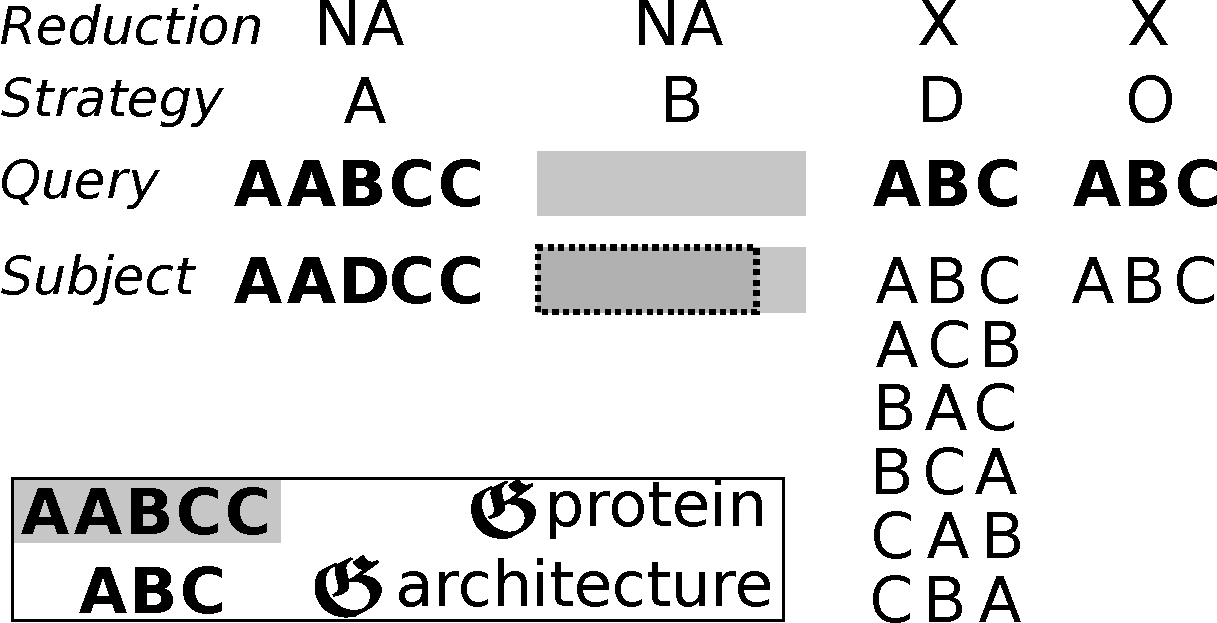
\includegraphics[scale=0.3]{figures/ABDO}%
\caption{Detail of comparisons between query and subject protein domains with 
	different pairwise comparisons: A, B, D, O.}
\label{fig:ABDO}
\end{figure}
%%%%%%%

Due the application of ABDO strategies was independently, it is possible to 
identify the relationships between the query species and the 
$\boldsymbol{\mathfrak{G}}$ species in the final set of immune system 
candidates through an architecture relationships. As shown in Figure 
~\ref{fig:FrecEstrat}A different combinations of possibles architecture 
comparisons strategies have been merged to four different sets, organized by the 
number of (ABDO) strategies that reported a successfully architecture 
comparison. Here, $1 = (A, D)$; $2 = (AB, AD, BD, DO)$; $3 = (ABD, ADO, BDO)$ 
and $4 = (ABDO)$; that is $10$ from $15$ possible combinations, because $ (AO, 
BO)$ always map to $ (ADO, BDO)$, due $D \subseteq O$ and additionally, $B$ has 
not been considered at all because this comparison does not represent a pure 
architecture relation, due complete sequence is used in the pairwise alignment 
against $\boldsymbol{\mathfrak{G}}$ protein sequences. 

%%%%Biological discussion about homology strategies of architectures
From each considered homology comparison, is possible to define their biological
meaning based on the predetermined constrains on the pairwise comparison. In this
case: \textsl{A} comparisons relies only in the arrangement of the protein domains as a 
string \cite{} (CITE RADS), this comparison takes into account similarity scores
between the protein domain models from Pfam. In this case, as shown in Figure
~\ref{fig:FrecEstrat}A, the high number of proteins corresponds to homodomain proteins
or proteins with only one annotated domain. This group are restricted to be detected
only by the A strategy, the other group, detected by only \textsl{D}, are proteins 
that reported the same number and type of protein domains, but does not conserve 
the arrangement respect to the query $\boldsymbol{\mathfrak{G}}$ architecture.
Next group, corresponds to proteins that have been detected by $2$ homology 
architecture methods. In this case, AB combines not only the domain arrangement detected
by RADS but also, local similarity scores between conserved regions are enough to report
high scores using \texttt{blast}.

\begin{sidewaystable}
\small
\centering
\begin{center}
\begin{tabular}{p{1cm}p{1.2cm}p{9cm}p{8cm}} 
\toprule
\textbf{Group} & \textbf{Strategy} & \textbf{Description}& \textbf{Example}\\
1 & A & Homodomain proteins or proteins with only one annotated domain & Q:ENSP00000332353 (hsa):
\textbf{PF02460,PF02460} \\ S:Boleac.CG.SB\_v3.S462.g10171.01.p 
(bole):\textbf{PF02460,PF02460}\\
& D & Proteins that reported the same number and type of domains, but does 
not conserve the arrangement respect to the query $\boldsymbol{\mathfrak{G}}$ architecture. &
Q:ENSP00000358159 (hsa): \textbf{PF00270;PF00271;PF02889} S:Moocci.CG.ELv1\_2.S377548.g10787.01.p (mlis)
: \textbf{PF02889;PF00270;PF00271} \\
\midrule
2 & AB & Combines both, domain arrangement detected by RADS and local similarity scores 
between conserved regions that are enough to report high scores using \texttt{blast}. & \\
& AD & Proteins that did not reported a strict domain arrangement, but all the same kind of
domains are reported. & Q:ENSP00000284320 (hsa):\textbf{PF00515,PF13181,PF13181,PF13181,PF13181}
S:PMI\_006942 (pami): \textbf{PF13181,PF00515} \\
& BD & Proteins that shares the same kinds of domains and also reported local similarities in overall
protein sequence in a pairwise alignment with \texttt{blastp} & Q:ENSP00000481034 (hsa): 
\textbf{PF07974,PF00008} S:ENSCSAVP00000003313 (cisa): 
\textbf{PF00008,PF00008,PF00008,PF00008,PF00008,PF00008,PF07974,PF00008,PF00008,PF07974,
PF07974,PF00008,PF00008,PF00008,PF00008,PF07974,PF00008,PF00008,PF00008,PF00008,PF00008,PF00008,
PF07974,PF00008,PF00008,PF00008,PF00008,PF00008,PF00008,PF00008,PF07974} \\
& DO & Proteins that reported the same arrangement and types of domains \TODO{I detected a bug in RADS
program. Seems that the architecture strategy somethimes missed true candidates, I wrote an email to
the people from RADS team} &   
Q:ENSP00000225614 (hsa): \textbf{PF10509,PF00288,PF08544} 
S:XP\_796432.3 (stpu): \textbf{PF10509,PF00288,PF08544}\\
\midrule
3 & ABD & Proteins that does not strictly share the same domain arrangement
but the architecture homology is enough to report a true candidates, this 
result is also supported by the pairwise comparison by \texttt{blast} and 
additionally, all the same protein families conserved between query and subject & 
Q:ENSMUSP00000118471 (mmu): \textbf{PF01421,PF00090,PF05986,PF00090,PF00090}
S:ENSCSAVP00000002867 (cisa): \textbf{PF01421,PF00090,PF05986}\\
& ADO & Proteins that strictly shares the same domain arrangement
and domain families. This group fails in \texttt{blast} searches, so
it means that homology is supported only by pure architecture. & 
Q:ENSP00000233330 (hsa): \textbf{PF08174,PF00169}
S:g15075.t1 (dive): \textbf{PF08174,PF00169}\\ 
& BDO & Those proteins would be the complete strategy, there is no reason
to discart A, because exits D and O. \TODO{I detected a bug in RADS program. Seems 
that the architecture strategy somethimes missed true candidates, I wrote an 
email to the people from RADS team} & 
Q:ENSP00000367421 (hsa): \textbf{PF02828,PF00595,PF07653,PF00625}
S:XP\_791632.3 (stpu): \textbf{PF02828,PF00595,PF07653,PF00625}\\
\midrule
4 & ABDO & Proteins that reported the most conserved architecture
and sequence homology. Those ones shares the same protein arrangement, 
types of domains and also local homology at pairwise comparisons. &
Q:ENSP00000358159 (hsa): \textbf{PF00270,PF00271,PF02889,PF00270,PF00271,PF02889}
S:GSOIDP00013289001 (oidi): \textbf{PF00270,PF00271,PF02889,PF00270,PF00271,PF02889}\\
\bottomrule
\end{tabular}
\end{center}
\caption{Biological meaning of combination of architecture strategies.}
\label{table:biologicalexplanation}
\end{sidewaystable}
%%%%

At the same time, this described distribution of relationships against 
$\boldsymbol{\mathfrak{G}}$ architectures shows a highest number of subjects that 
have been detected as innate immune system candidates by only $1$ architecture 
strategy, most of them with A. The number of candidates that have been detected with 
all the strategies (set $4$) reported frequencies $\leq 3100$ proteins on the 
subject species, reporting the highest distribution on the specie \textit{D.\ 
rerio}. This group represents, along all the comparisons the most conserved 
set of immune proteins respect to the defined $\boldsymbol{\mathfrak{G}}$. 

Considering in overall the immune system proteins along all the studied 
species, it is possible to identify the proportion of shared innate immune 
system proteins respect to $\boldsymbol{\mathfrak{G}}$ species (Figure 
~\ref{fig:FrecEstrat}B). Mainly those relationships have been detected with human 
and mouse proteins, as described earlier those $\boldsymbol{\mathfrak{G}}$ 
species reported the most frequent proteins in $\boldsymbol{\mathfrak{G}}$ set. 
%Why Cisa has less mmu shared proteins respect to Ciro? They are sister species!

\begin{figure}[ht!]
\centering
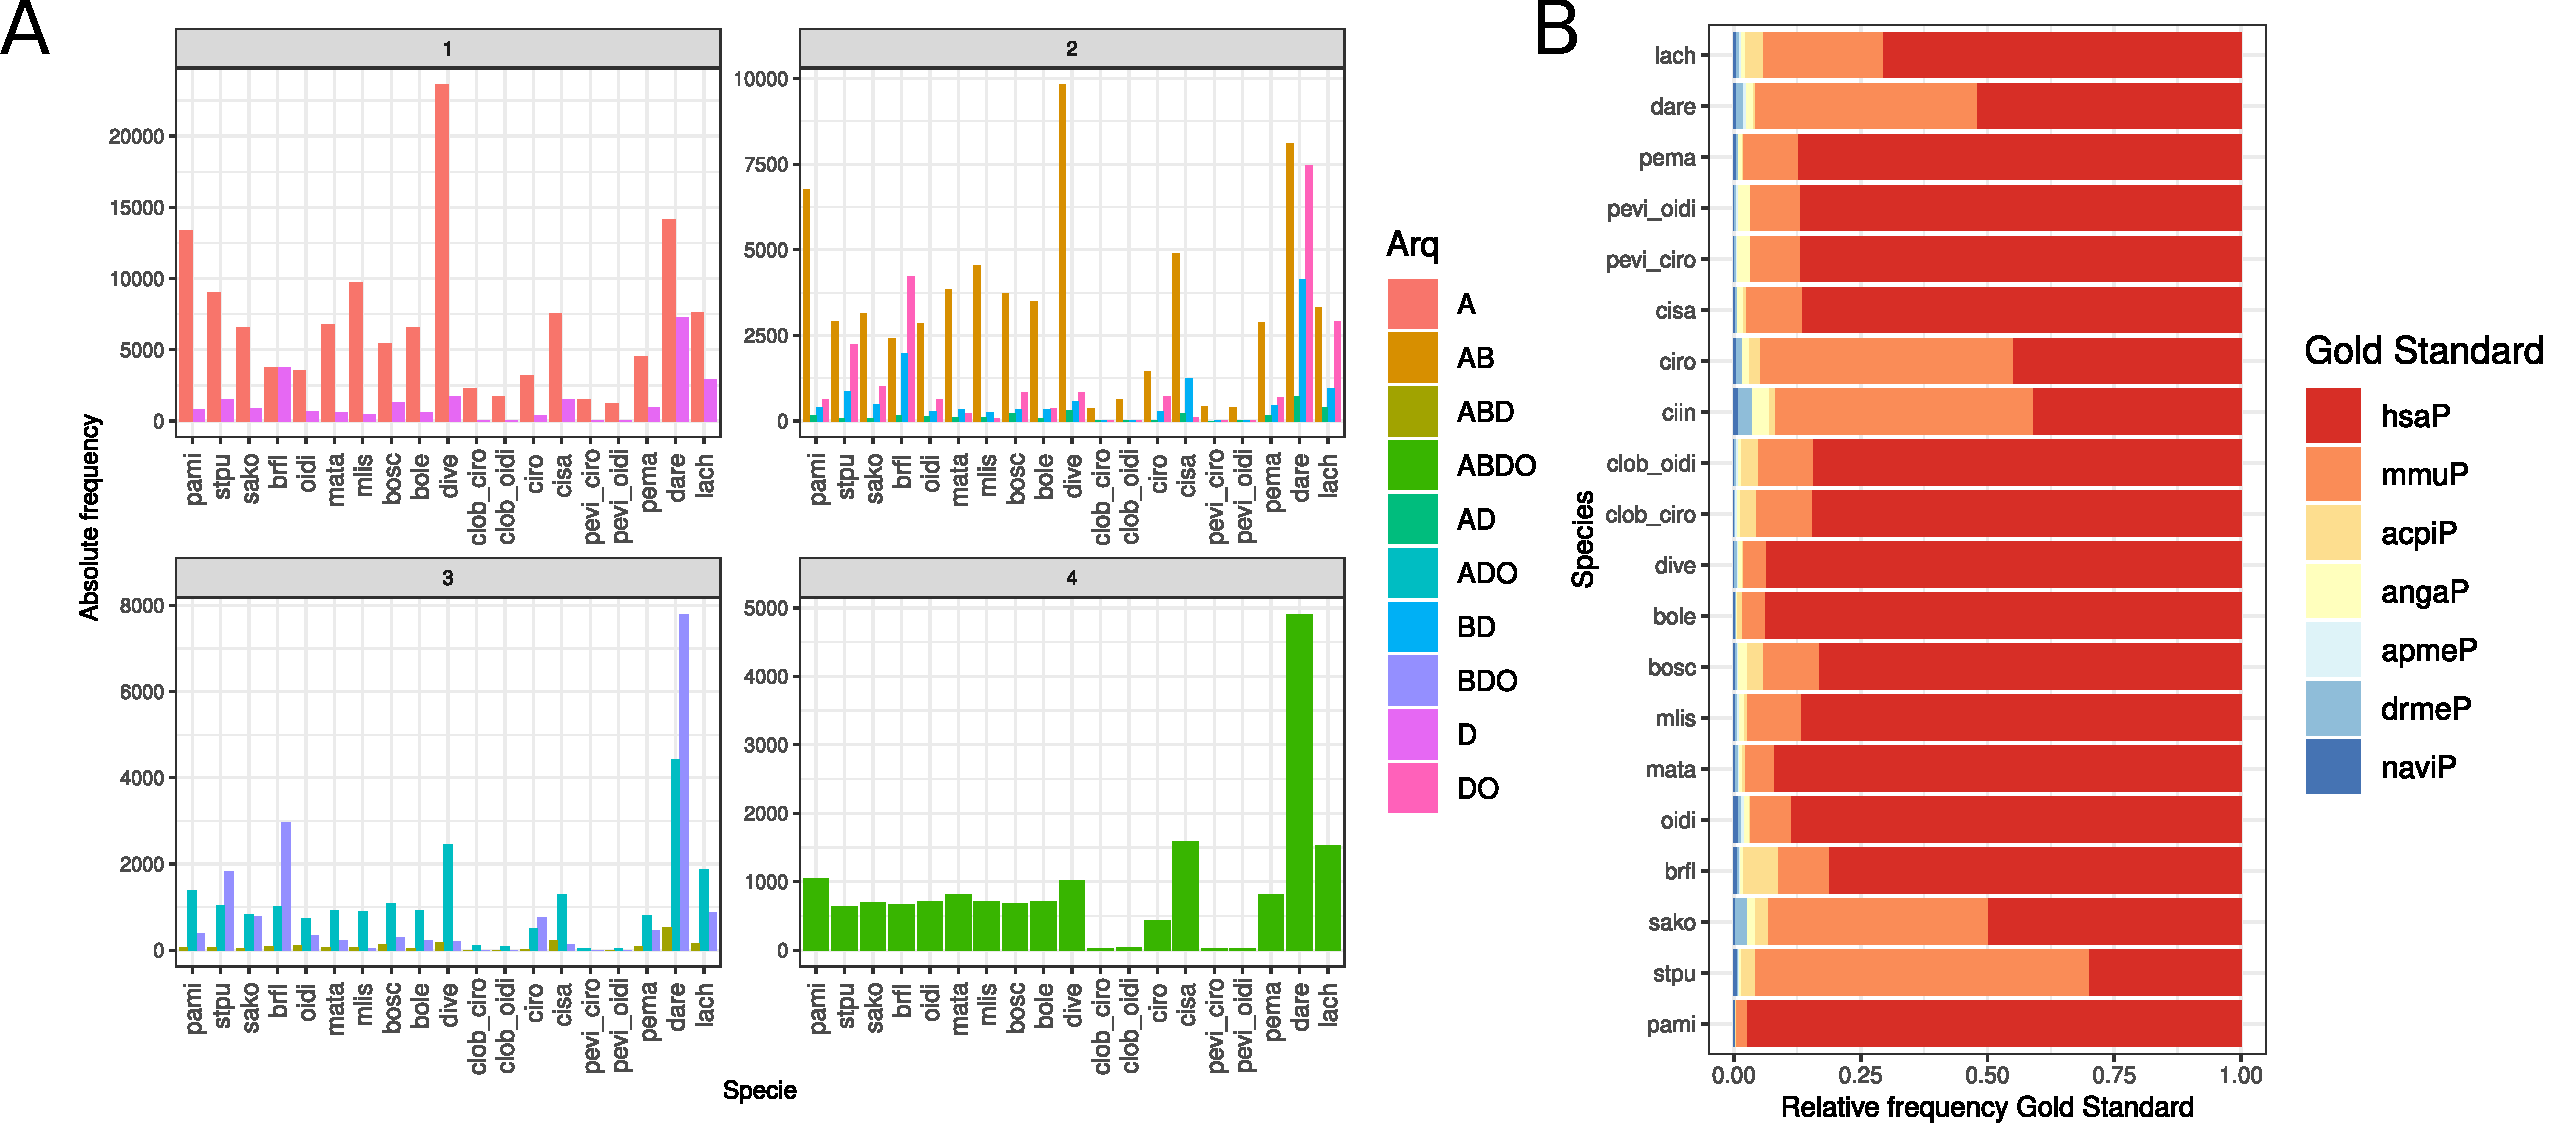
\includegraphics[scale=0.43]{figures/unitedComparedGOLD}%
\caption{
\textbf{A}Frequency of detected proteins with defined architecture
comparison strategies classified according to the number of possible combinations of 
architecture strategies (described in more detail in main text), 
against $\boldsymbol{\mathfrak{G}}$. \textbf{B} Mean shared proportion 
homology architecture against gold standard species. \textsf{naviP=}\textit{N.\ 
vitripennis}, \textsf{apmeP=}\textit{A.\ mellifera}, \textsf{drmeP=}\textit{D.\ 
melanogaster}, \textsf{angaP=}\textit{A.\ gambiae} and 
\textsf{acpiP=}\textit{A.\ pisum}; and Mammals: 
\textsf{mmuP=}\textit{M.\ musculus} and \textsf{hsaP=}\textit{H.\ sapiens}.
}
\label{fig:FrecEstrat}
\end{figure}


\subsection*{Relationships between Innate Immune system candidates} 
\label{Orthology}

Obtaining the protein domain architectures after their detection by ABDO 
strategies, the distribution of the number of domains was studied (Figure 
~\ref{fig:domainDistr}A). All the studied organisms were grouped in $5$ 
defined taxonomical clades as follows: \textbf{Echi} = Echinodermata, 
\textbf{Hemi} = Hemichordata, \textbf{Ceph} = Cephalochordata, \textbf{Tuni} = 
Tunicata and \textbf{Vert} = Vertebrata, following the sub-phylum assignment on 
Additional File 1:Table 1. It was possible to identify a high number of 
proteins that only reported $1$ protein domain type (homodomain proteins).
Despite the similarity of this results along all clades, distribution 
from \textsl{B.\ floridae} (Cephalochordata) showed also higher number of 
proteins with $2$ and $3$ types of domains with similar numbers as reported 
on vertebrates; but not in echinoderms, hemichordates and tunicates, that 
showed similar density distributions. Also, few proteins are composed by more 
than $5$ different types of domains, but the current distributions shows, in 
all clades, a very long heavy tails with \TODO{$\ge 20$ domains types}.

Meanwhile, Figures~\ref{fig:domainDistr}B and C, shows the distribution of 
protein architectures on homodomain and heterodomain proteins along studied 
species, respectively. For homodomain proteins, $2304$ domain architectures 
were detected along innate immune proteins in echinoderms ($54.1$\%), 
hemichordates ($51.3$\%), cephalochordates ($37.0$\%), tunicates ($43.1$\%) and 
vertebrates ($52.9$\%). This distribution also shows a high variation in 
total number of architectures of one type of domain in echinoderms and 
tunicates, respect to vertebrates (an excluding Hemichordates and 
Cephalochordates that have $n=1$). \TODO{Please, explain this with a more 
detailed plot or data for tunicates and echinoderms.}.

In this homodomain set, the most frequent protein architecture with 
current annotation from \texttt{Pfam} database is: Rhodopsin-like receptor 
(PF00001) for echinoderms, hemichordates and vertebrates, while for 
Cephalochordata was Cytochrome P450 (PF00067) and for tunicates the Protein 
Kinase domain (PF00069). 

A number of $1936$ heterodomain architectures have been detected along the set 
of proteins. Specifically, for all clades, was possible to calculate 
the percentage of found architectures respect to the total number of 
heterodomain architectures for all clades: echinoderms ($42.3$\%), 
hemichordates ($45.0$\%), cephalochordates ($47.1$\%), tunicates 
($22.5$\%) and vertebrates ($50.8$\%). In more detail, 
Figure~\ref{fig:domainDistr}C shows the average of found protein architectures 
along all the clades. Both, the presence percentage and the average number of 
architectures shows a reduced number of found architectures on tunicates 
proteins, in comparison to other species of chordates and the outgroup species. 
Also, a high variability is evident for the complete Tunicata clade. \TODO{Maybe 
make a stat test?, please make a plot!}.  

As a complement for heterodomain proteins, Figure~\ref{fig:domainDistr}D 
represent the top $5$ proteins architectures domains along all defined clades. 
This distribution is dominated by only $10$ domains that are spanned along 
the protein architectures. By this way, the most frequent domain is an 
Immunoglobulin domain (Ig 3, PF13927), in vertebrates, tunicates and 
echinoderms. In relation with this domain, in echinoderms and hemichordates a 
frequent domain is the Immunoglobulin I-set domain (PF07679). Leucine-rich 
repeats (PF13855), related with protein-protein interactions are frequent in 
vertebrates and cephalochordates and additionally related with this funcion, 
Ankyrin repeats (PF12796) and the Calcium-binding EGF domain (PF07645) have 
been detected in this list. The most conserved along those clades are: P-kinase 
(PF00069) and related domains as: Tyrosin kinase (PF07714), and even Pleckstrin 
homology domain (PF00169). 

\TODO{When the architecture distribution is considered, the most frequent along 
all species are described on Table~\ref{tab:mostConservedArch}. Change 
this table describing by specie, clade or even describe the matrix based on 1:1 
orthologous proteins.}

\begin{figure}[ht!]
\centering
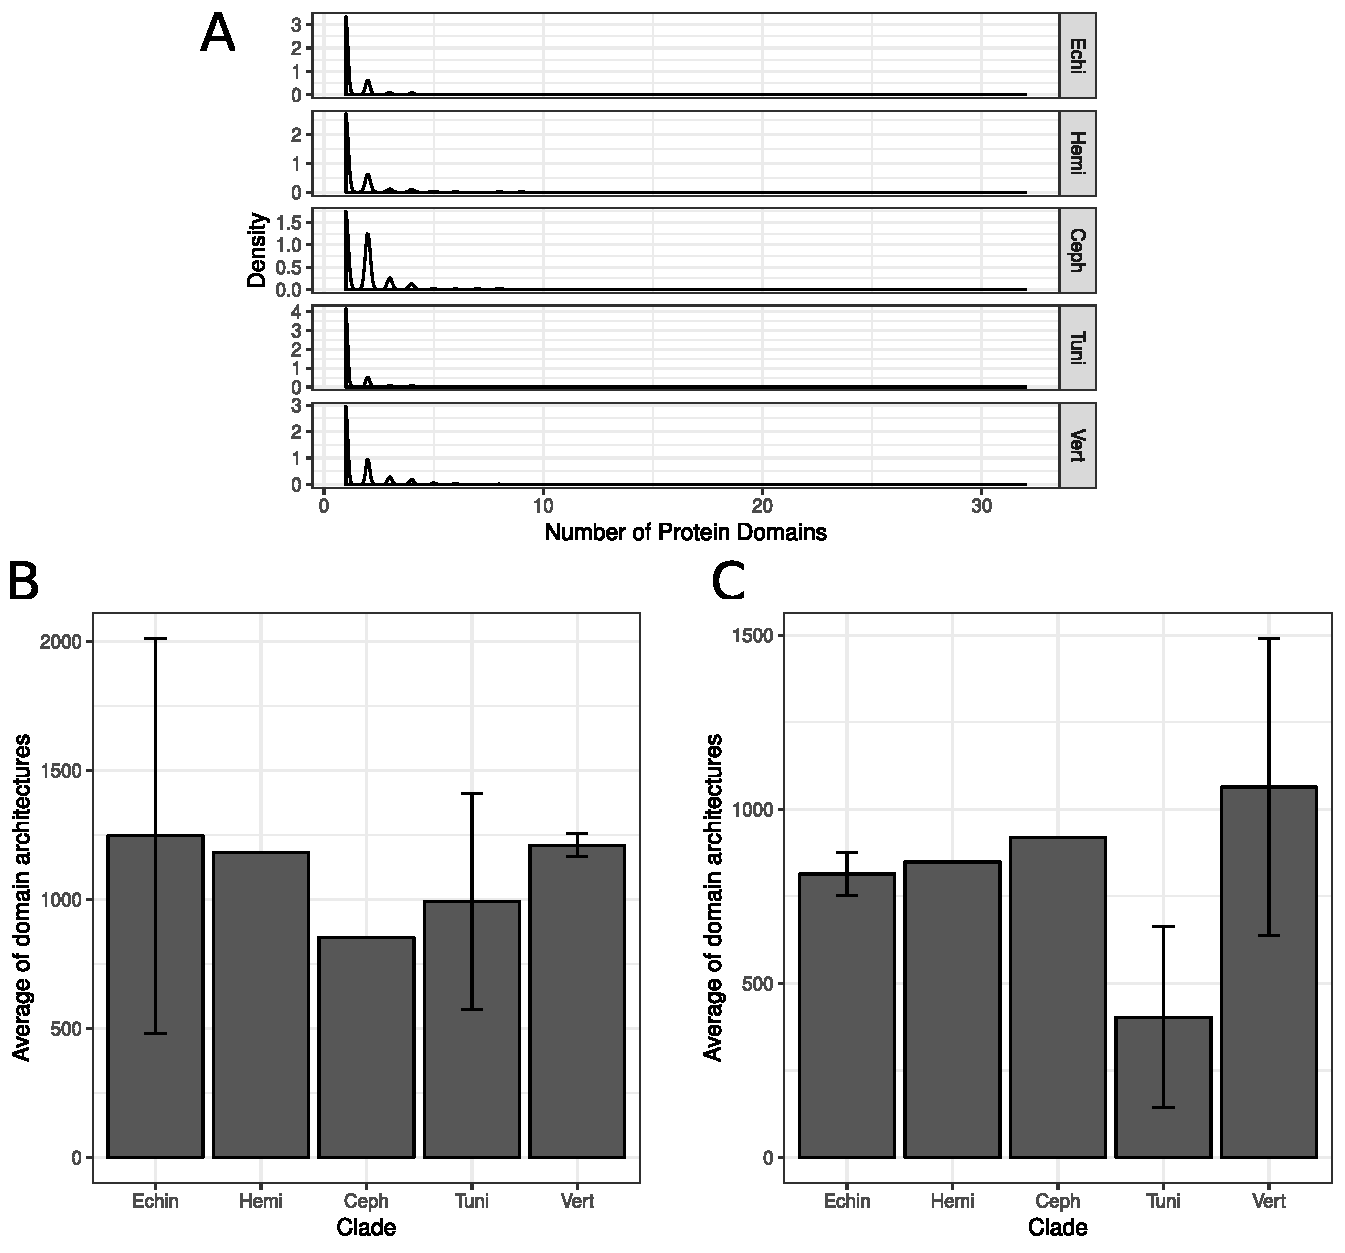
\includegraphics[scale=0.53]{figures/completeDistributionDomains} \\
%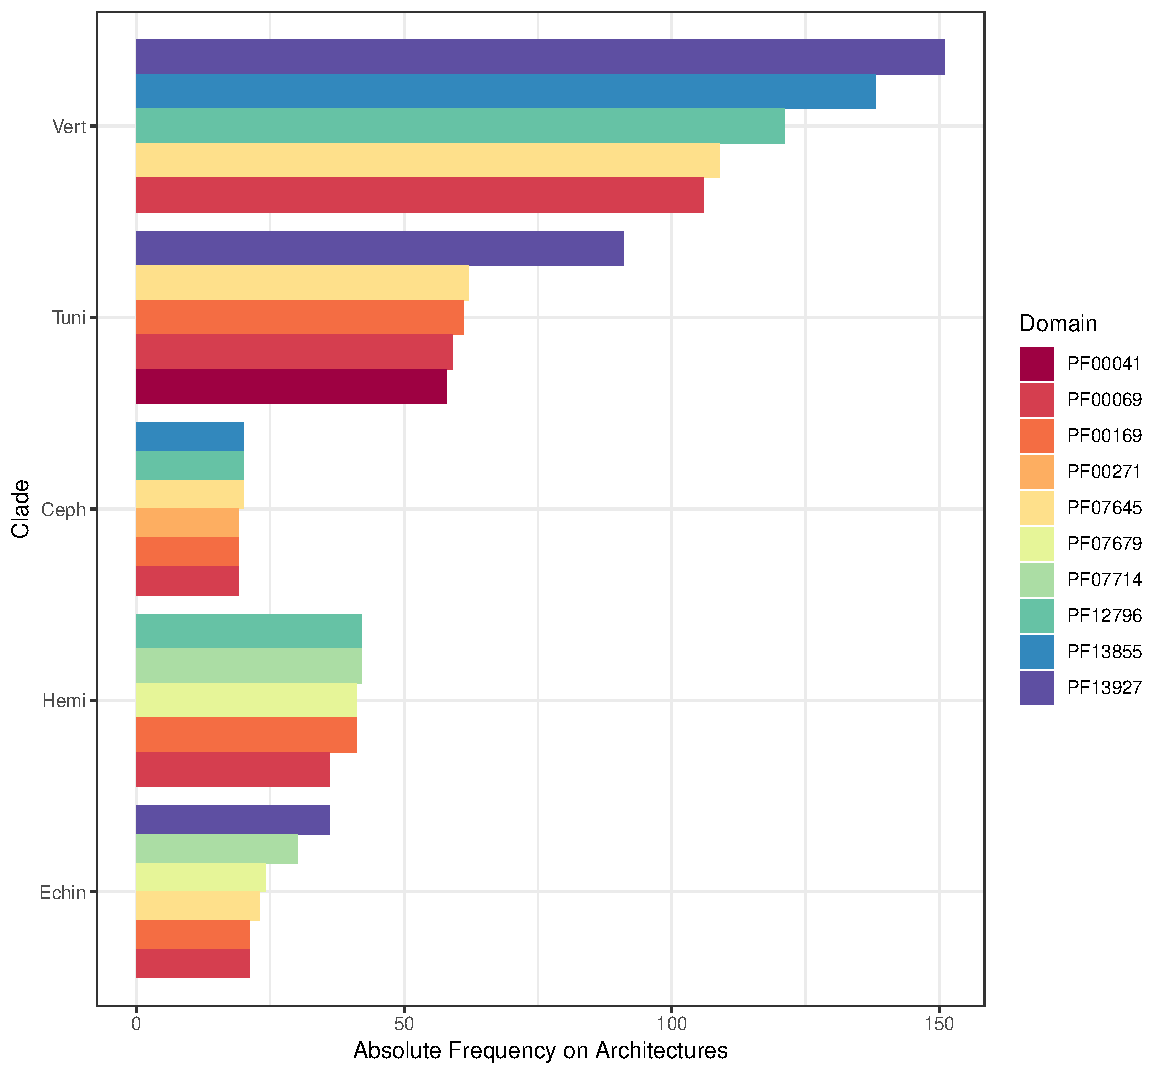
\includegraphics[scale=0.38]{figures/heterodomains_distr}
\caption{
\textbf{A} Homodomain architecture distribution. 
\textbf{B} Multidomain architecture distribution. \textbf{Echi:} 
Echinodermata, \textbf{Hemi:} Hemichordata, \textbf{Ceph:} Cephalochordata, 
\textbf{Tuni:} Tunicata and \textbf{Vert:} Vertebrata.
}
\label{fig:domainDistr}
\end{figure}

\begin{table}[ht!]
\caption{Most conserved architectures along studied species. \TODO{Maybe reeplace 
this table for one more complete table with the most conserved along species? Additional file?}}
\begin{center}
\begin{tabular}{llp{4cm}}
\toprule
\textbf{Architecture} & \textbf{Annotation} & \textbf{References}\\
\midrule
PF00134,PF16899 & Cyclin\_N,Cyclin\_C\_2 & NA\\
PF00651,PF07707 &  BTB,BACK & 
\url{https://www.ncbi.nlm.nih.gov/pubmed/15544948}\\
PF00688,PF00019 & TGFb\_propeptide,TGF\_beta & 
\url{https://www.sciencedirect.com/science/article/pii/S0145305X03001812?via\%3Dihub}\\
PF04851,PF00271 & ResIII,Helicase\_C & NA\\
PF07707,PF01344 & BACK,Kelch\_1 & NA\\
PF15227,PF00643 & zf-C3HC4\_4,zf-B\_box & NA \\
\bottomrule
\end{tabular}
\label{tab:mostConservedArch}
\end{center}
\end{table}

Once protein candidates were detected by ABDO strategies on studied species, 
a further step is the identification of the biological relevance of the 
new detected protein candidates. Applying a clustering strategy was
possible to identify the intrinsic relationships between 
$\boldsymbol{\mathfrak{G}}$ and the new identified proteins, based on common 
protein domain architectures. In this way $4240$ groups were created and to 
access for orthology relationships with described methodology with \texttt{ProteinOrtho}.
The first step to study those relations is the identification of orthologous (1:1) 
or co-orthologous (1:many or many:many) groups. In this way, a total of $27311$ 
relations were detected, from them: $53.13$\% reports 1:1 relationships, while
co-orthologs are represented by $46.87$\%. Based on the 1:1 orthology relations and 
their relationship with protein architectures a matrix was generated with the number 
of proteins for each specie. In this way, was identified $2740$ architectures related
with 1:1 relations and was possible to identify $38$ architectures
%(23 architectures conserved + 15 conserved in all species and at least one of 
%the calculated gene model ciro or oidi for clob or pevi) 
that are conserved in all species (\TODO{Describe all at new Supp. File?}). 
Most of this conserved set of architectures corresponds to homodomain proteins, 
except for $3$ heterodomain architectures (PF00134:PF16899,PF04851:PF00271 
and PF07707:PF01344). At the same time, based in the same matrix it is possible 
to reconstruct the architecture domain history along all studied species by Dollo 
parsimony \cite{} with \texttt{Count}\cite{csuros2010}. 

As represented on Figure~\ref{fig:dollooneone},  a set of $1477$ architectures 
are shared in the base of the \TODO{Deuterostomia?} and in both clades: 
chordates and ambulacrarians report only gains (g) events. In this way, at the 
base of Chordata $1619$ architectures have been partially loss (l) in Cephalochordata
(l:986) in comparison to Olfactores (l:20, g:276) that reported an additional 
set of gained architectures. In the divergence between \textit{Tunicata} 
and \textit{Vertebrata}, both clades reported specific gains and losses, but with a 
higher number of losses that could be traced in the base of vertebrates (l:483, g:62).
Gain and loss in tunicates could be traced (g:18,l:145), but not at the same magnitude
as occurred in vertebrates, with $1748$ architectures. More than $70.25$\% of those architectures have been lost in \textit{O. dioica} (Appendicularians) and also reporting 
a very few number of gains (g:7). \TODO{The clade that groups} \textsl{Stolidobranchia, Phlebobranchia and Aplousobranchia} increased the total number of architectures. 
In comparison, more loss events have been detected in the clade (Phlebobranchia +
Aplousobranchia) (g:17, l:386) than Stolidobranchia (g:34, l:232). In overall through
those clades is important to note that Aplousobranchia reported 
between almost twice loss events (g:6,l:523) than Phlebobranchia (g:2, l:283) and Stolidobranchia (g:34, l:232). At the same time, exists a high number of lost 
architectures in species where \textit{de novo} gene prediction was predicted (with 
gene models from \textit{C.\ robusta} and \textit{O.\ dioica} using \texttt{GeneID}). At 
the end, final numbers of orthologous architectures are reported for each 
specie. Specie-specific or clade-specific gains resulted for \textit{P.\ miniata} 
the highest number of specific architectures. In terms of numbers, 
Stolidobranchia reported, in average, biggest values of architectures ($972.5$) 
than Aplousobranchia ($634$) and Phlebobranchia ($617$), despite the high number 
of gains registered on \textit{C.\ savignyi} (g:37, l:284), in general at the 
base of the Stolidobranchia happened a similar gain event (g:34, l:232). 
Finally, inside vertebrates the highest number of architectures are present on 
\textit{D.\ rerio}, not only the specie-specific gain events (g:86,l:319), but also 
gains at the base of Osteichthyes (g:102, l:178).

As mentioned earlier, is possible divide the architecture domains into: homodomain 
and heterodomain. Figure~\ref{fig:domainDistr}A shows that homodomain proteins 
are the most frequent in all clades in comparison to heterodomain proteins, 
except for cephalochordates. In order to analyze the evolutionary history of 
heterodomain orthologous proteins (1:1), the evolutionary history reconstruction 
using Dollo parsimony was applied as described earlier (Figure~\ref{fig:dollooneoneheterodomain}). A $437$ of $1133$ architectures were shared 
between Deuterostomata, again showing gain events at Ambulacraria (g:29) and 
Chordata (g:113). Cepahlochordata lost about $42$\% of the ancestral architectures 
for chordates, while in Olfactores predominate gain events (g:130, l:9). The 
ancestral number of heterodomain architectures in Tunicata are $595$, specifically 
in \textit{O.\ dioica} report the most higher loss of domains $73.9$\%. 
At thre same time, Stolidobranchia shows higher heterodomain architectures in 
comparison to Phlebobranchia and Aplousobranchia. A number of $526$ heterodomain
 architectures are at the base of vertebrates, and about $48,8$\% are lost in 
 \textsl{P.\ marinus} (g:8, l:257). In contrast, Osteichthyes reported few loss and 
 10 times gain events (g:80, l:30). At the end, not only in vertebrates, but in all 
analyzed species, \textit{D.\ rerio} report the biggest number of heterodomain 
architectures ($525$).

\begin{figure}[ht!]
\centering
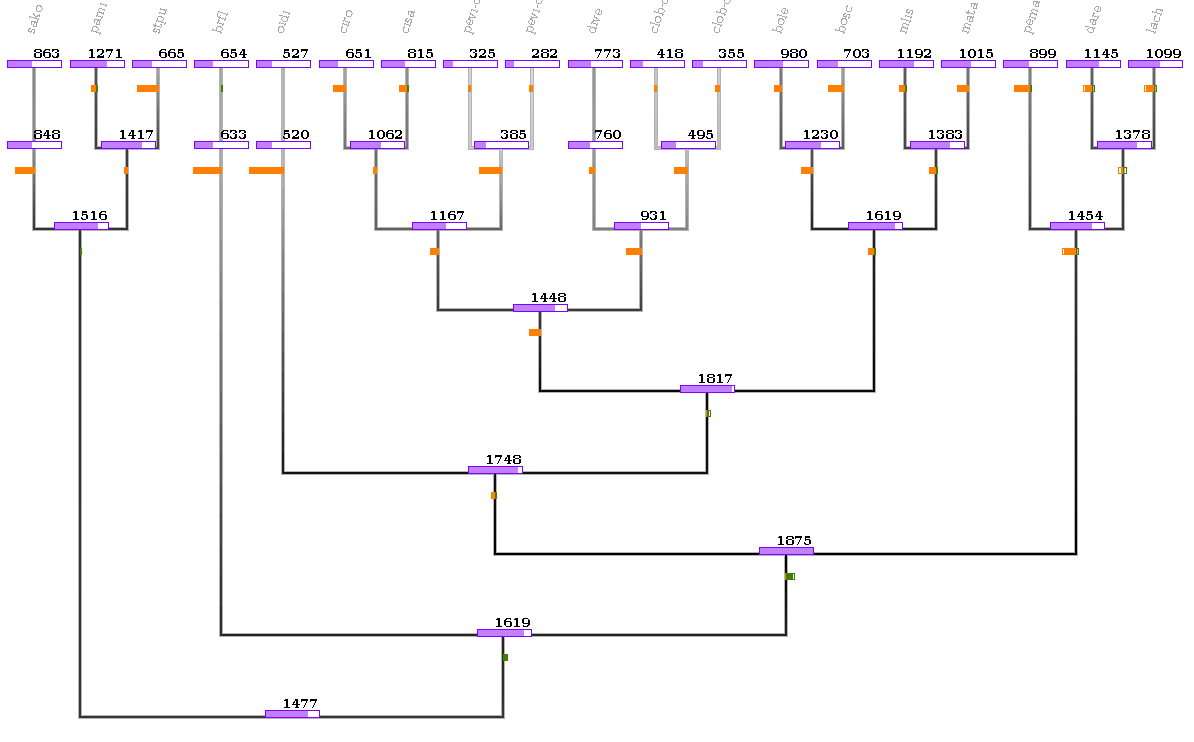
\includegraphics[scale=0.53]{figures/provisionalDollo} \\
\caption{Evolutionary history of 1:1 orthologous protein architectures in 
Deuterostomata. \TODO{This is a temporal image, while I'm sure about numbers}}
\label{fig:dollooneone}
\end{figure}

\begin{figure}[ht!]
\centering
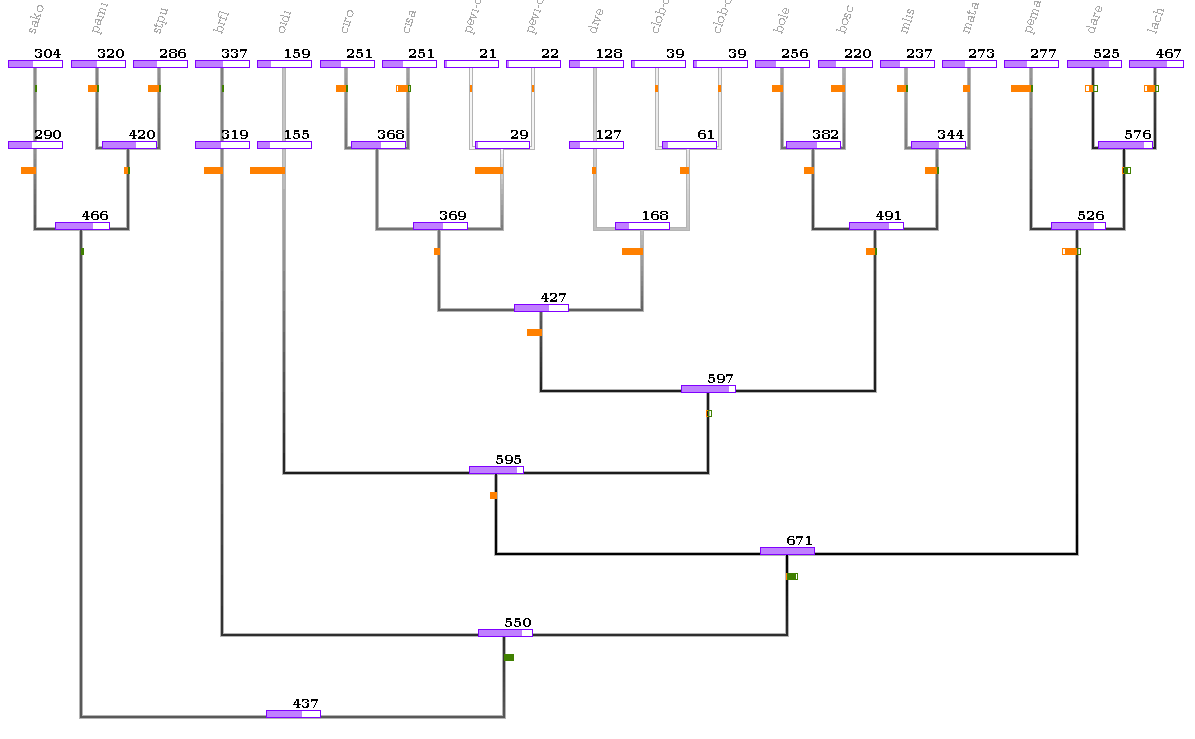
\includegraphics[scale=0.53]{figures/provisionalDolloHeterodomains} \\
\caption{Evolutionary history of 1:1 orthologous \textbf{heterodomain} protein 
architectures in Deuterostomata.}
\label{fig:dollooneoneheterodomain}
\end{figure}

In the same way, from the $27311$ relations that have been detected, 
those ones that have been classified as 1:1 orthology ($14510$) reported a 
sub-set of $2732$ groups have at least one $\boldsymbol{\mathfrak{G}}$ protein.
From co-orthologous comparisons ($12801$) were detected and a subset 
of $5293$ have at least one $\boldsymbol{\mathfrak{G}}$ protein. 
For those sub-sets with $\boldsymbol{\mathfrak{G}}$ proteins was possible 
to retrieve the \texttt{Interpro} annotation using \texttt{biomaRt}. 
\TODO{Final tables are reported in Additional Files 3 (oneone\_heterodomains\_annotation\_proteins.txt, oneone\_homodomains\_annotation\_proteins.txt)}.

\TODO{TODO:}
\begin{itemize}
\item \TODO{In this case, I have the interpro annotation for a given architecture based
on the golden protein ($\boldsymbol{\mathfrak{G}}$) which have a 1:1 relationship. Just
reporting those data? or is more convenient to plot by some way?}
\item \TODO{Because the paper is about innate immune system, I was looking for 
categories which I could classify the final architectures. I have found a nice classification
specifically for tunicates on \url{https://www.ncbi.nlm.nih.gov/pmc/articles/PMC5465252/pdf/fimmu-08-00674.pdf} but I have to take some examples for each category and look it into
the found candidates. Another option is on this systematic revision of domains: \url{https://www.sciencedirect.com/science/article/pii/S0378111918311119?via\%3Dihub}.}.
\item \TODO{Dollo parsimony could be applied for analize gain and loss of protein architectures?.}
\item \TODO{I could represent the protein architectures as drawings of the proteins, or a comparison between species, but for the most important ones in innate immune system, there is lot of information.}
\item \TODO{I would like to report the ABDO method. I have the program, mainly Perl scripts and glue code in bash or maybe in a server?}
\end{itemize}

\section*{Conclusions}

\bibliographystyle{abbrvnat}
\bibliography{biblio,otherbibio}

\end{document}
